\documentclass[times,11pt]{ACME2015article}
\usepackage{amsmath,amssymb,amsthm,mathrsfs,graphicx}
\usepackage{natbib,subfigure}
\usepackage{titlesec}
\usepackage{multirow}

\setlength{\parindent}{0pt}
\setlength{\parskip}{5pt plus 2pt minus 1 pt}

\topmargin  -25mm
\evensidemargin 0mm
\oddsidemargin  0mm
\textwidth  160mm
\textheight 267mm
%\renewcommand{\baselinestretch}{1.0}
\frenchspacing
\sloppy
\titlespacing{\section}{0pt}{\parskip}{0.01\parskip}

\newcommand{\mb}{\mathbf}
%%%%%%%%%%%%%%%%%%%%%%%%%%%%%%%%%%%%%%%%%%%%%%%%%%%%%%%%%%%%%%%%%%%%%%%
\begin {document}
\pagestyle{empty}

\begin{flushright}
{\fontsize{8}{10}
\it Proceedings of the 23$^\mathrm{rd}$ UK Conference of the\\
Association for Computational Mechanics in Engineering\\
8 - 10 April 2015, Swansea University, Swansea\\} \vskip 1.2 cm
\end{flushright}

\begin{center}
{\fontsize{14}{20}\bf Computation of resonant modes in cavities with a Discontinuous Galerkin time domain approach
}\end{center}


\begin{center}
\textbf{M. Dawson, R. Sevilla, O. Hassan and K. Morgan}\\
\end{center}

\begin{center}
{\fontsize{10}{12}
Zienkiewicz Centre for Computational Engineering, College of Engineering, Swansea University, Swansea, Wales, UK SA2 8PP\\
}\end{center}

\begin{center}
\{743587,R.Sevilla,O.Hassan,K.Morgan\}@swansea.ac.uk\\
\end{center}
%
\begin{center}
\textbf{ABSTRACT}\\[1mm]
\end{center}
%

\begin{normalsize}
We present a method of obtaining frequency domain quantities of an electromagnetic resonator, such as the frequency spectrum, quality factors, resonant frequencies and the associated mode shapes, using a parallelised Discontinuous Galerkin solver with explicit time marching. The method is validated using a 2D free-space cavity with analytically known resonant frequencies. The relative error in resonant frequency is quantified and we demonstrate a faster convergence of error, using the filter diagonalisation method (FDM), than with the traditional fast Fourier transform (FFT). The implementation of material dispersion in the solver is validated using a 2D dispersive cavity with known analytical solution.
\end{normalsize}

\textbf{\textit{Key Words:}} {\it Finite Element, Discontinuous Galerkin, Electromagnetics, Resonant Cavities, Time Domain }
%
\\
\section{Introduction}
Recent advances in manufacturing techniques, such as electron beam lithography, make it possible to manufacture resonant cavities on the scale of the wavelength of light. These nanoresonators, key components in nanolasers, can have many desirable qualities such as well defined resonant frequencies and high quality factors \cite{busch2011discontinuous}. However, the typical scale and the geometric complexity introduce several challenges for numerical simulation.

The behaviour of these resonators is described by Maxwells' equations of classical electromagnetics. For dispersive materials, an auxiliary ordinary differential equation based on the Drude models \cite{taflove1995computational} is coupled to the Maxwell system. Frequency domain solvers are traditionally employed to find the resonant frequencies and associated modes, but as the scale and geometric complexity of the devices increase, the large eigenvalue system that must be solved becomes computationally prohibitive.

We propose to use the Discontinuous Galerkin (DG) method with explicit time marching, which only requires solving a block diagonal system of equations for each timestep \cite{sevilla2014use}. The frequency spectrum, resonant frequencies and quality factors can then be recovered by a Fourier transform of the time domain solution.

\section{DG solution of the transient Maxwell's equations in dispersive media}

Maxwell's equations of classical electromagnetics and the auxiliary ordinary different equation required for dispersive media can be written in linear, dimensionless, conservation form as
\begin{equation}\label{maxwell-eqtns}
\frac{\partial \, \mb{U}}{\partial t} + \sum_{k=1}^{nsd} \frac { \partial \, \mb{F}_k(\mb{U}) }{ \partial x_k } = \mb{S}\,(\mb{U}) \: ,
\end{equation}

%The behaviour of nano-scale resonators can be simulated using Maxwells' equations of classical electromagnetics. For metallic devices an additional coupled Auxiliary Differential Equation (ADE) is required to accounts for the frequency dependence of the material parameters due to finite time required for materials to respond to applied fields using the Drude model of solids. The system of equations to be solved can be written in linear, dimensionless conservation form as


% where $nsd$ denotes the number of spatial dimensions. The vector of unknowns, $\mb{U}$, is given by $\mb{U}_1 = \begin{pmatrix} \epsilon E_1 & \epsilon E_2 & \epsilon E_3 & \mu H_1 & \mu H_2 &  \mu H_3 & J_1 &  J_2 & J_3 \end{pmatrix}^T$, the flux vectors, $\mb{F}_k$, are given by $\mb{F}_1 = \begin{pmatrix} 0 & H_3 & -H_2 & 0 & -E_3 & E_2 & 0 &  0 & 0 \end{pmatrix}^T$, $\mb{F}_2 = \begin{pmatrix} - H_3 & 0 & H_1 & E_3 & 0 & -E_1 & 0 &  0 & 0 \end{pmatrix}^T$ and $\mb{F}_3 = \begin{pmatrix} H_2 & -H_1 & 0 & -E_2 & E_1 & 0 & 0 &  0 & 0 \end{pmatrix}^T$ and the source $\mb{S}$ is given by $\mb{S} = \begin{pmatrix} 0 & 0 & 0 & 0 & 0 & 0 & \omega^2_d E_1 - \gamma_d J_1 &  \omega^2_d E_2 - \gamma_d J_2 & \omega^2_d E_3 - \gamma_d J_3 \end{pmatrix}^T$.

where $nsd$ denotes the number of spatial dimensions. The vector of unknowns, $\mb{U}$, the flux vectors, $\mb{F}_k$, and the source $\mathbf{S}$ are given by

\begin{equation*}
\begin{array}{ccccc}
\mb{U}_1 = \begin{pmatrix} \epsilon E_1 \\ \epsilon E_2 \\ \epsilon E_3 \\ \mu H_1 \\ \mu H_2 \\  \mu H_3 \\ J_1 \\  J_2 \\ J_3 \end{pmatrix} ,
&
\mb{F}_1 = \begin{pmatrix} 0 \\ H_3 \\ -H_2 \\ 0 \\ -E_3 \\ E_2 \\ 0 \\  0 \\ 0 \end{pmatrix} ,
&
\mb{F}_2 = \begin{pmatrix} - H_3 \\ 0 \\ H_1 \\ E_3 \\ 0 \\ -E_1 \\ 0 \\  0 \\ 0 \end{pmatrix} ,
&
\mb{F}_3 = \begin{pmatrix} H_2 \\ -H_1 \\ 0 \\ -E_2 \\ E_1 \\ 0 \\ 0 \\  0 \\ 0 \end{pmatrix} ,
&
\mb{S} = \begin{pmatrix} 0 \\ 0 \\ 0 \\ 0 \\ 0 \\ 0 \\ \omega^2 \, E_1 - \gamma J_1 \\  \omega^2 \, E_2 - \gamma J_2 \\ \omega^2 \, E_3 - \gamma J_3 \end{pmatrix} ,
\end{array}
\:
\end{equation*}

where $E_k$, $H_k$ and $J_k$ are the $k$th spatial components of the dimensionless intensity vectors of electric field, magnetic field and the polarisation current respectively. The material parameters $\epsilon$, $\mu$, $\omega$ and $\gamma$ are the electric permittivity, magnetic permeability, plasma frequency and electron damping coefficient respectively.

We discretise the computational domain $\Omega$ on an unstructured mesh. The DG weak formulation \cite{hesthaven2007nodal} of \eqref{maxwell-eqtns} on an element $\Omega_e$ can then be written as

\begin{equation*}
\int_{\Omega_{e}} \mb{W} \, \frac{\partial \, \mb{U}_e }{ \partial t } d \Omega + \int_{\Omega_e} \mb{W} \cdot \left( \sum_k^{nsd} \frac{ \partial \mb{F}_k\,(\mb{U}_e) }{ \partial x_k} - \mb{S}\,(\mb{U}_e) \right) d \Omega + \int_{\partial \Omega_e} \mb{W} \cdot \mb{A}_n^{-} \, \llbracket \mb{U}_e \rrbracket \; d \Gamma_e = 0 \; ,
\end{equation*}

where $\mb{U}_e$ denotes the solution vector restricted to the element $\Omega_e$, $\mb{W}$ is a vector of test functions and $ \llbracket \mb{U}_e \rrbracket = \mb{U}_e - \mb{U}_{out}$ denotes the jump of the solution across the element boundary $\Gamma_e$. The boundary term, derived after introducing the numerical flux on the boundary and using a flux-splitting technique, results in

\begin{equation*}
\mb{A}_n^{-} \, \llbracket \mb{U}_e \rrbracket = \frac{1}{2} \begin{pmatrix} -\mb{n} \times \llbracket \mb{H} \rrbracket + \mb{n} \times ( \mb{n} \times \llbracket \mb{E} \rrbracket ) \\ \mb{n} \times \llbracket \mb{E} \rrbracket + \mb{n} \times ( \mb{n} \times \llbracket \mb{H} \rrbracket ) \\
\mb{0}_{3}
 \end{pmatrix}
 \; ,
\end{equation*}

where $\mb{n}$ is the outward unit normal of the element and $\mb{0}_{3}$ is a zero vector of length 3. After introducing the approximation of the solution and using a Galerkin formulation, the following system of ordinary differential equations is obtained,

\begin{equation*}
\mb{M} \frac{d \boldsymbol{U}}{dt} + \mb{R}\,(\boldsymbol{U}) = \mb{0} \; ,
\end{equation*}

where $\boldsymbol{U}$ is the vector of nodal values, $\mb{M}$ is the block diagonal mass matrix and $\mb{R}\,(\boldsymbol{U})$ is the residual vector. The system of ordinary differential equations is advanced in time using a fourth-order explicit Runge-Kutta method.

\section{Computation of resonant frequencies}

The engineering quantities of interest in cavities are usually the resonant frequencies, associated modes and quality factors. In order to obtain these quantities using a time domain solver, the electromagnetic field is first excited by introducing an initial condition or a source in the domain (Figure \ref{frequency_schematic-init-cond}). As the solution is advanced in time, its value is monitored at each timestep for a given period of time, $T$ (Figure \ref{frequency_schematic-signal}). Using the fast Fourier transform, or more sophisticated techniques, we can then obtain the frequency spectrum (Figure \ref{frequency_schematic-spectrum}) from the monitored solution. The resonant frequencies of the cavity can be obtained from the locations of peaks in the frequency spectrum by curve-fitting and the quality factors from the width of the peaks. Mode shapes can be obtained by running the time domain simulation with the resonant frequency as an input.

\begin{figure}[htbp!]
 \centering
% 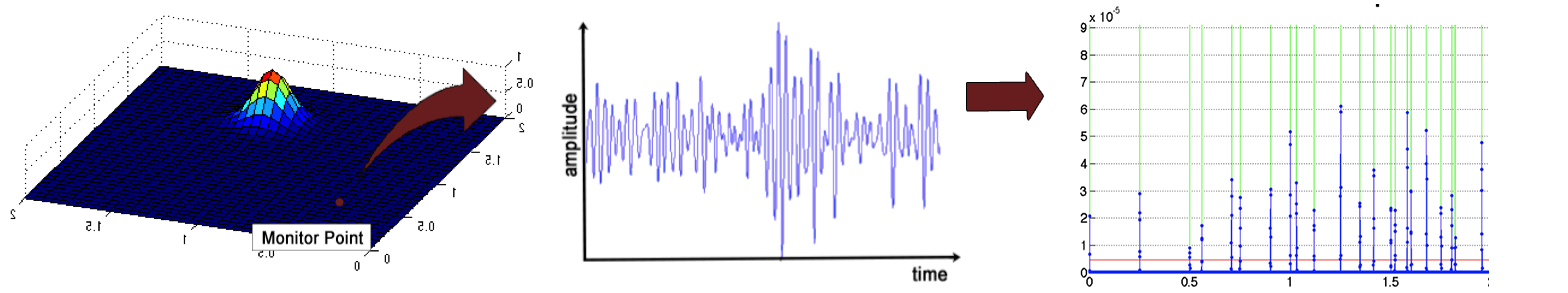
\includegraphics[width=\textwidth]{Figures/SpectrumSchematic}
\subfigure[Gaussian initial condition]{
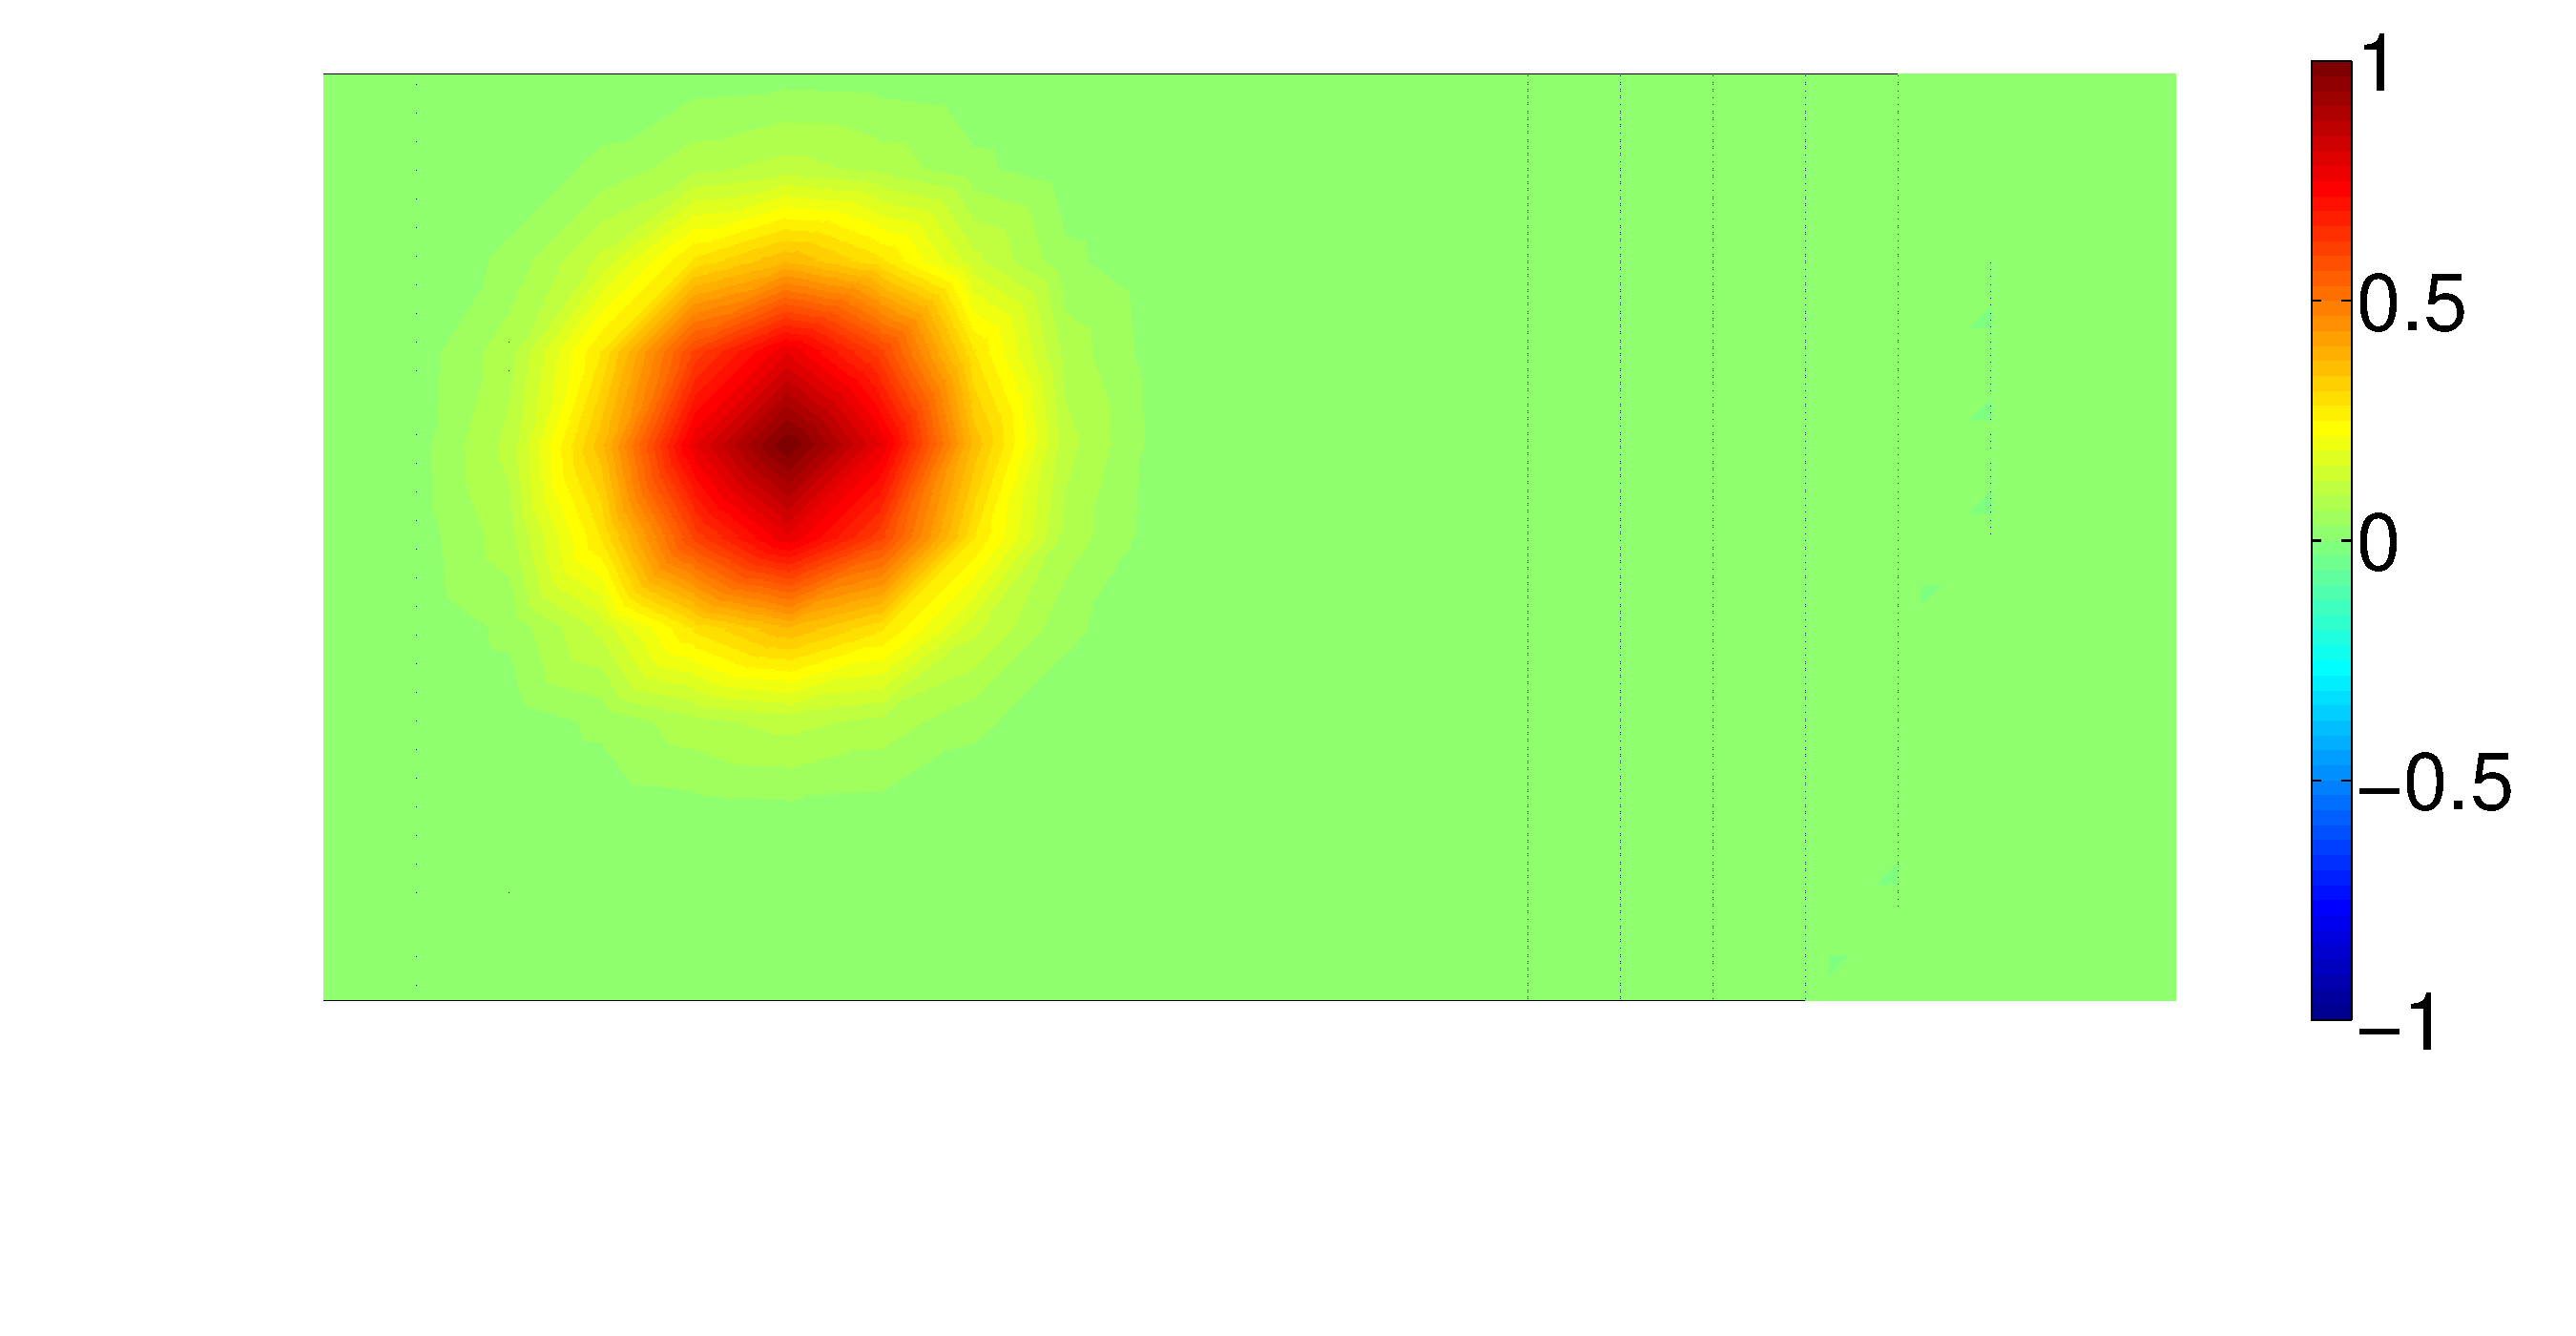
\includegraphics[height=3.5cm]{Figures/GaussianInitCond/GaussianInitCond}
\label{frequency_schematic-init-cond}
} \subfigure[Solution monitored at a point]{
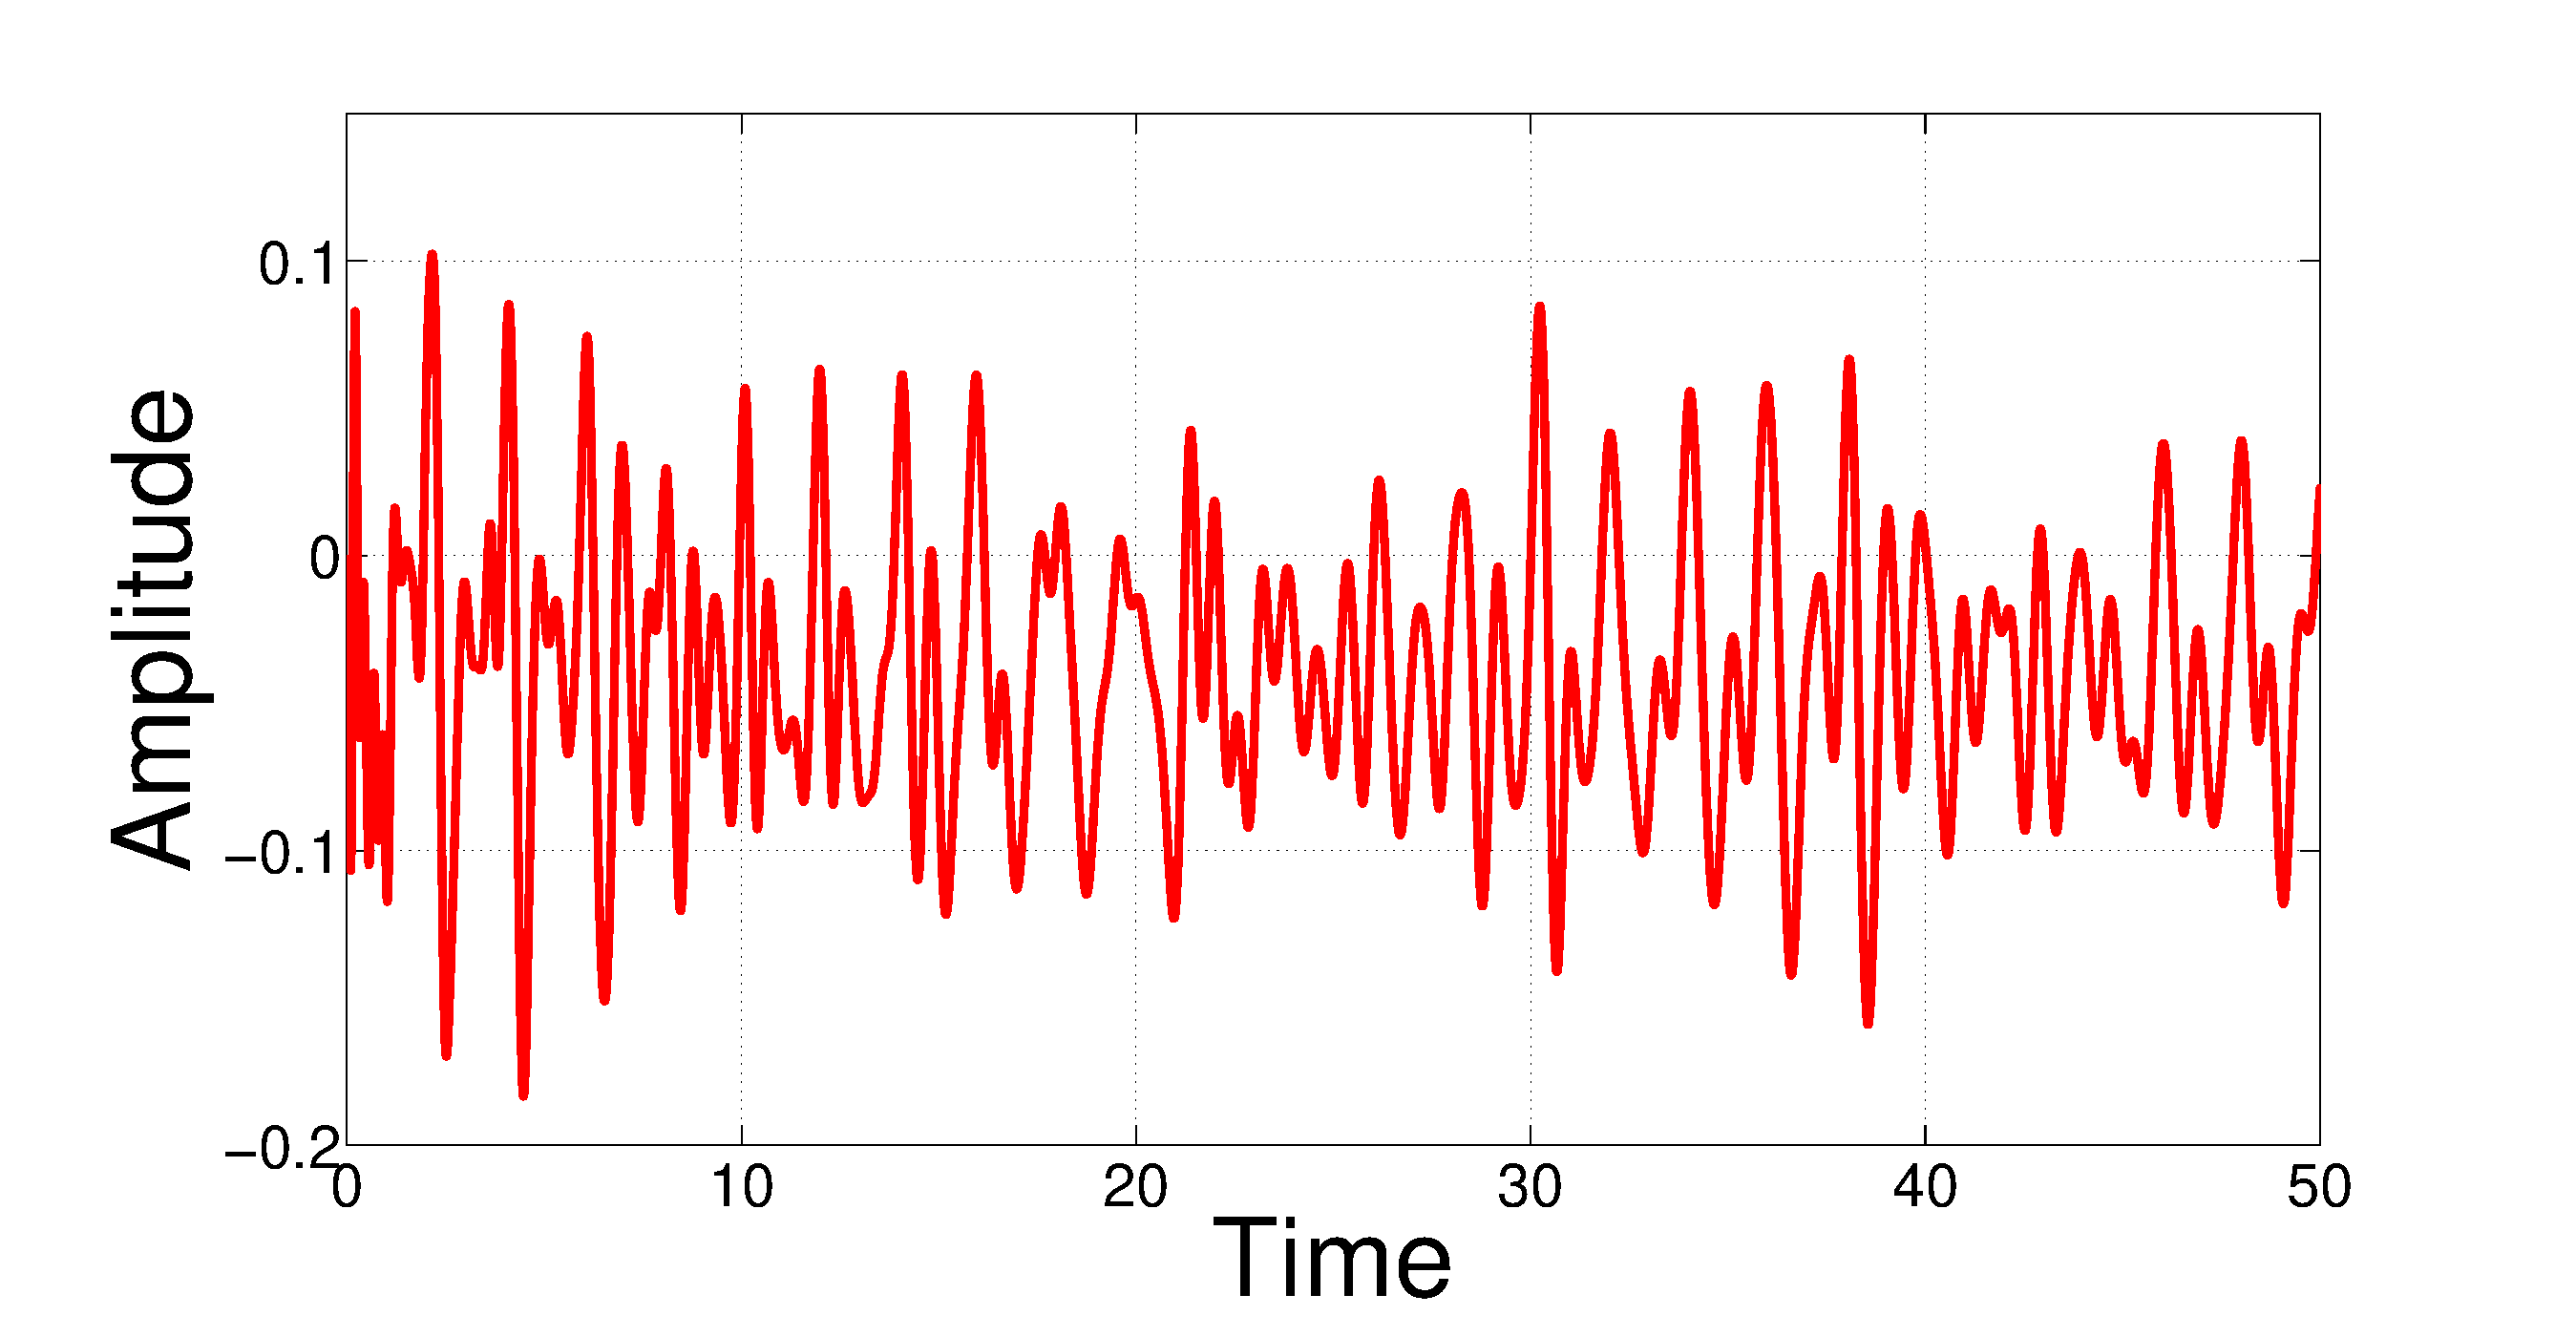
\includegraphics[height=3.5cm]{Figures/Spectrum/Signal}
\label{frequency_schematic-signal}
} \subfigure[Eigenspectrum obtained by FFT]{
\label{frequency_schematic-spectrum}
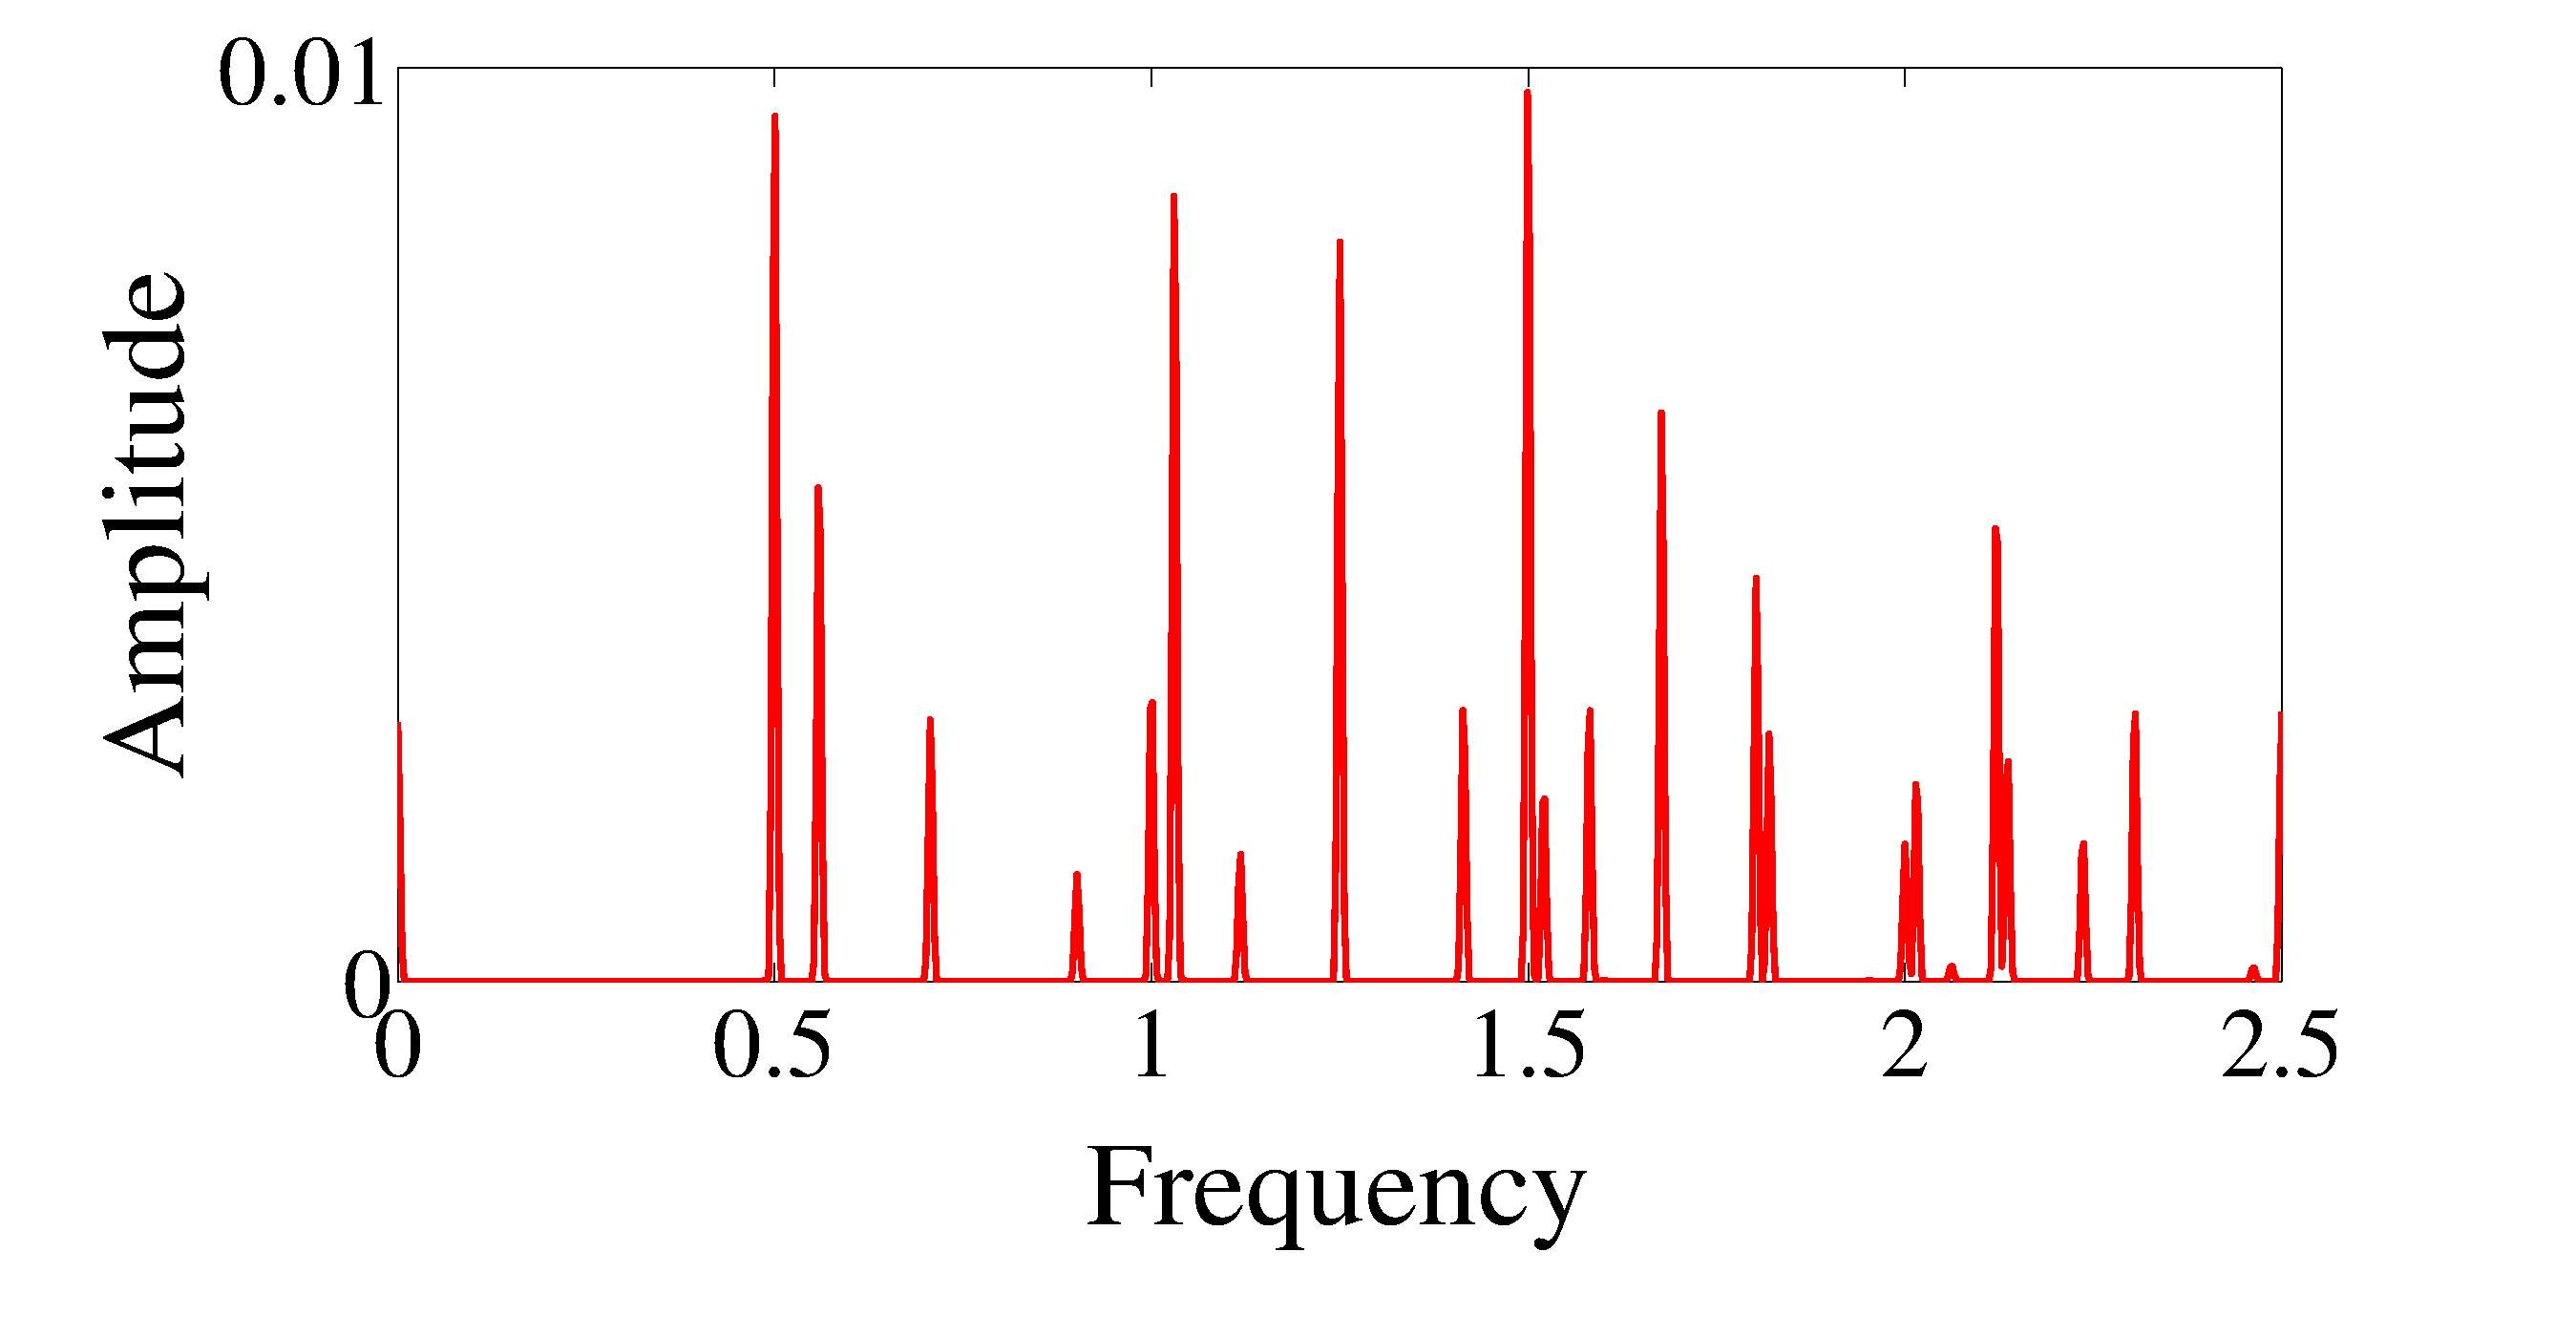
\includegraphics[height=3.5cm]{Figures/Spectrum/Spectrum-coarse}
}
\caption{Steps required to find the frequency spectrum and resonant frequencies shown for a 2D rectangular cavity.}
\end{figure}

The error in frequency is inversely proportional to $T$, and the highest frequency is inversely proportional to the simulation timestep. The main limitation of the proposed approach is therefore the need for longer periods in order to minimise the error in the obtained resonant frequencies. To overcome this issue we considered the filter diagonalisation method \cite{Mandelshtam1997} (FDM) which gives a much better accuracy than FFT in a significantly shorter time period. % as shown in Figure \ref{FFT-FDM-comparison}.

To further improve the performance of the proposed approach, the relative ease of parallelisation of the DG method is exploited to achieve the long periods required in reasonable computational time. The solver has been parallelised using MPI and the implementation and performance has been validated using two- and three-dimensional test cases. 

%\begin{figure}[htbp!]
% \centering
% 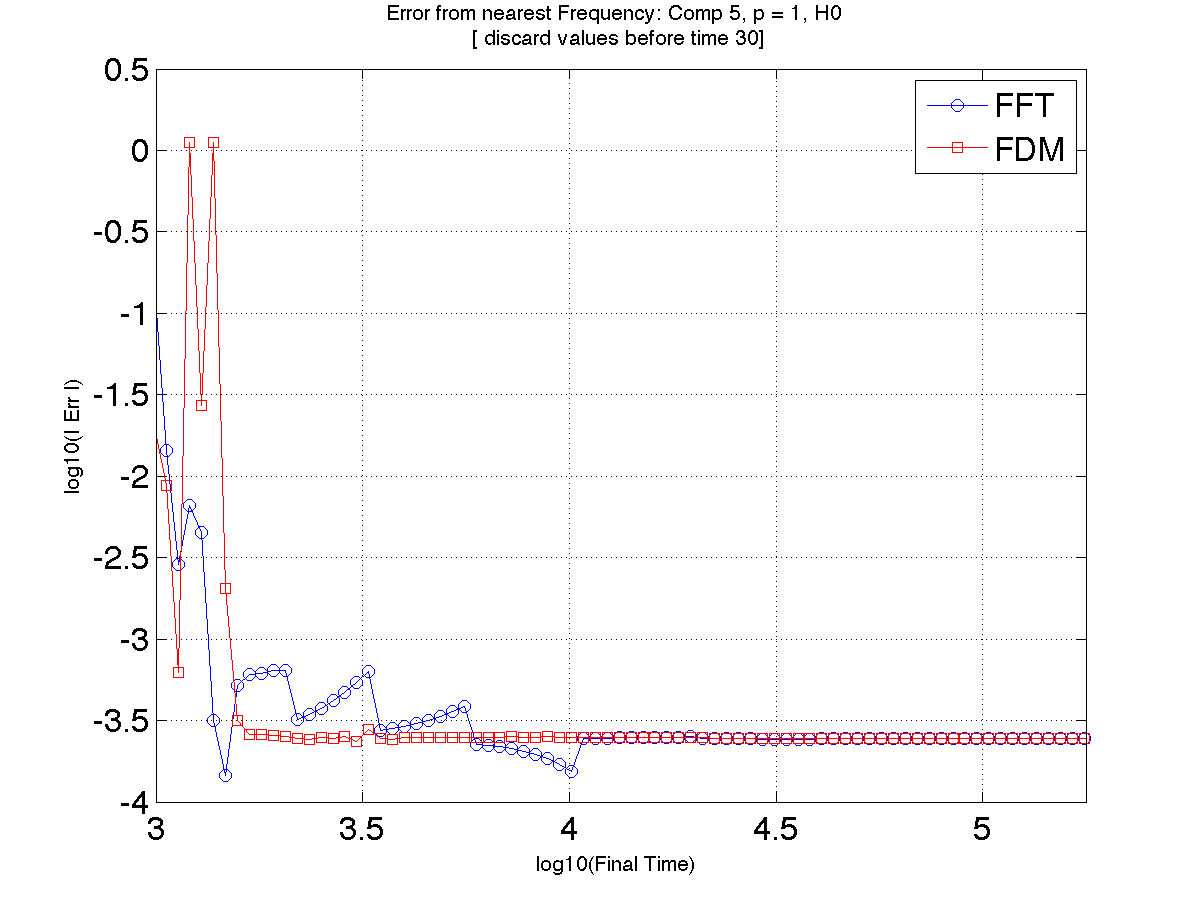
\includegraphics[height=4cm]{Figures/FDMvsFFT/FDMvsFDM_H0_p1_U5_freq3}
% \caption{Comparison of convergence of the relative error in frequency for FDM method and FFT method fitted with a spline}
% \label{FFT-FDM-comparison}
%\end{figure}

\section{Numerical Results}

%\subsection{Free Space Cavity}

The first example presented is a rectangular 2D non-dispersive free-space cavity ($\epsilon = \mu = 1$, $\omega = \gamma = 0$) surrounded by a perfect electric conductor (PEC) with a width twice its length. Analytical expressions for the resonant frequencies of this cavity are known \cite{pozar2006microwave}. Figure \ref{freeSpaceConvergence} shows the relative error in the resonant frequencies converging as expected with $T$. The final value is the error due to the spatial discretisation of the domain, which decreases with mesh refinement. The error using FDM can be seen to converge almost an order of magnitude quicker than FFT, as Figure \ref{FDMvsFFT} shows.

%0.19141 0.034593 500
%-0.71722 -0.31595 500
%0.043817 0.35284 500
%0.70799 0.34823 500
%-0.1499 -0.26982 500
%0.55117 -0.13145 500
%-0.52811 0.16374 500

\begin{figure}[htbp!]
 \centering
 \subfigure[]{
 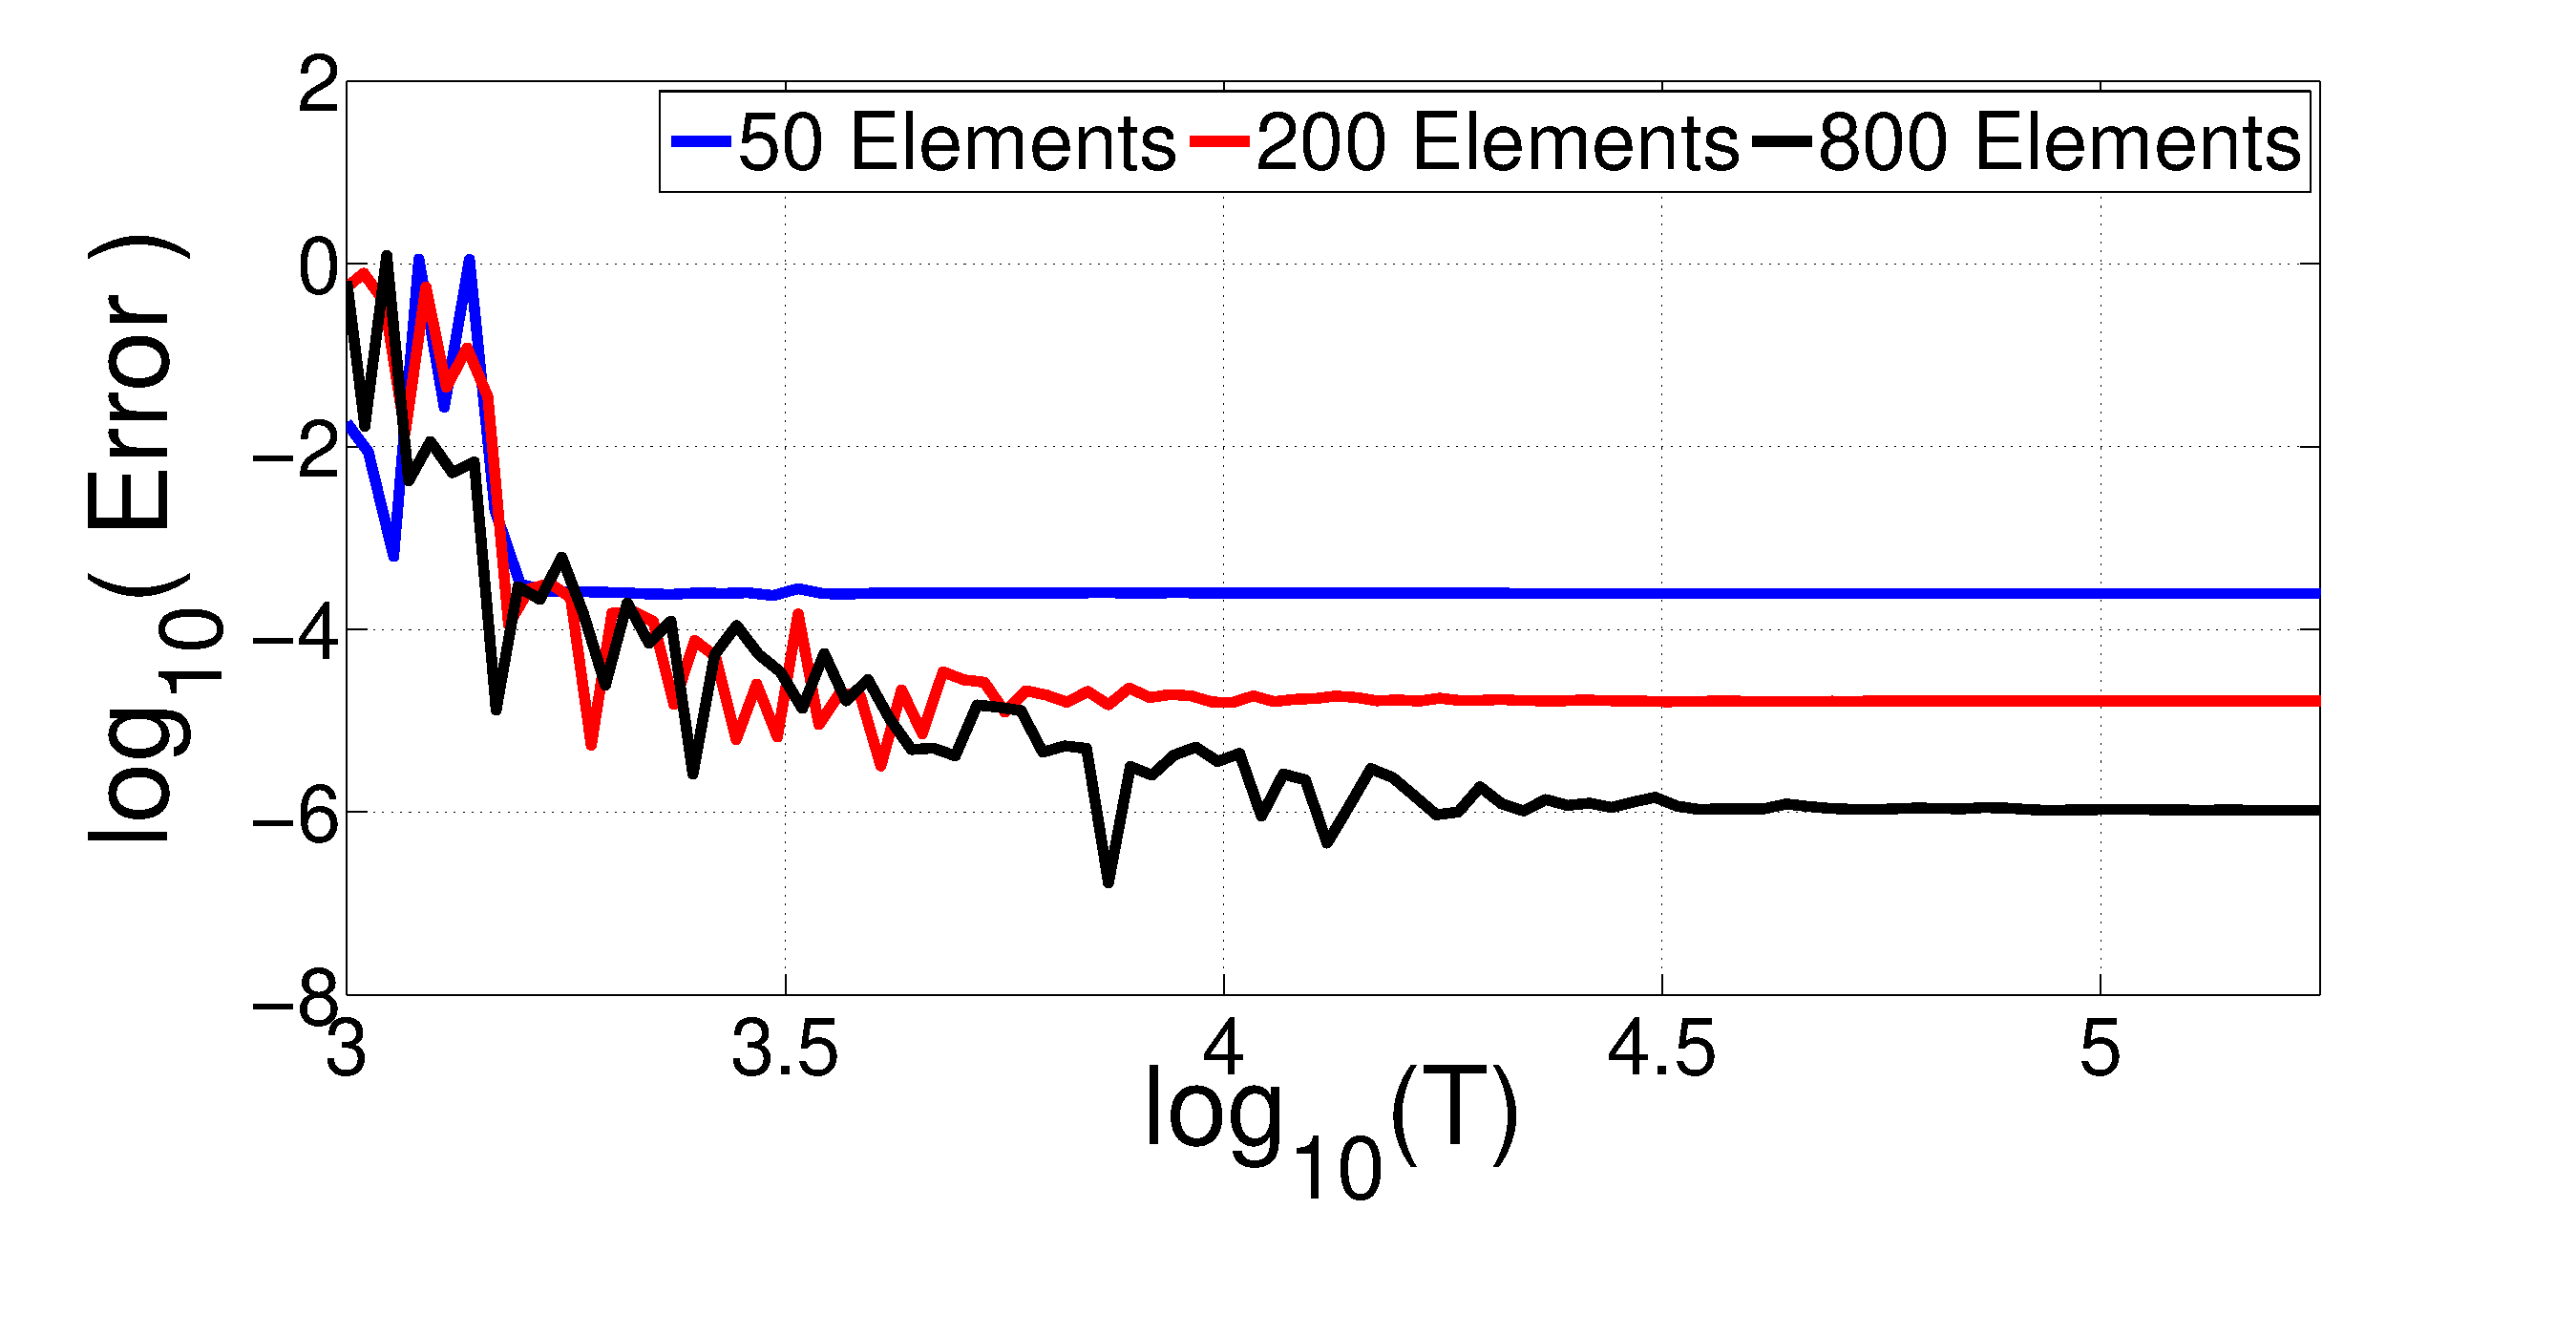
\includegraphics[width=0.485\textwidth]{Figures/FDMEvolutionWithPeriod/FDM_p1_U5_freq3_edited_2}
\label{freeSpaceConvergence}
 } \subfigure[]{
 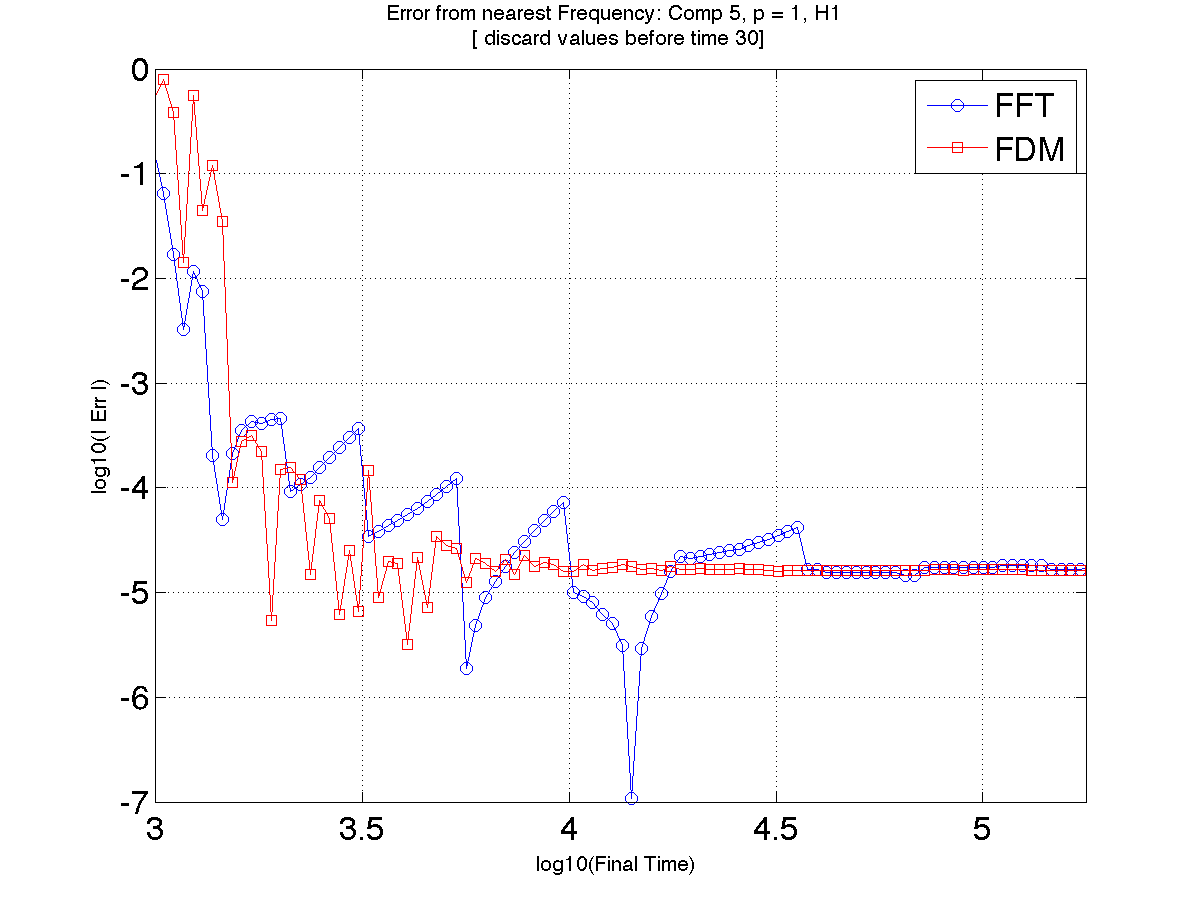
\includegraphics[width=0.485\textwidth]{Figures/FDMvsFFT/FDM+FDM_H1_p1_U5_freq3}
 \label{FDMvsFFT}
 }
 \caption{ (a) Convergence of the relative error in calculated resonant frequencies with increasing period T for three different meshes in a free space cavity. (b) Comparison of convergence with period obtained with FDM and FFT. }
\end{figure}

% \begin{figure}
% \centering
% 
% \begin{tabular}{ll}
% \subfigure[]{
%   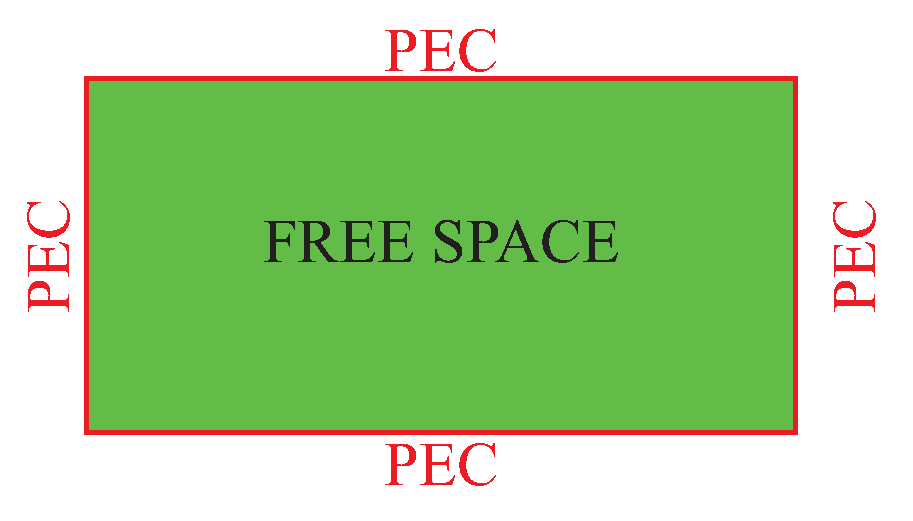
\includegraphics[width=0.3\textwidth]{Figures/Schematics/CavitySchematic}
% }
% &
% \multirow{-2}[0]{*}[57pt]{
%   \subfigure[]{
%     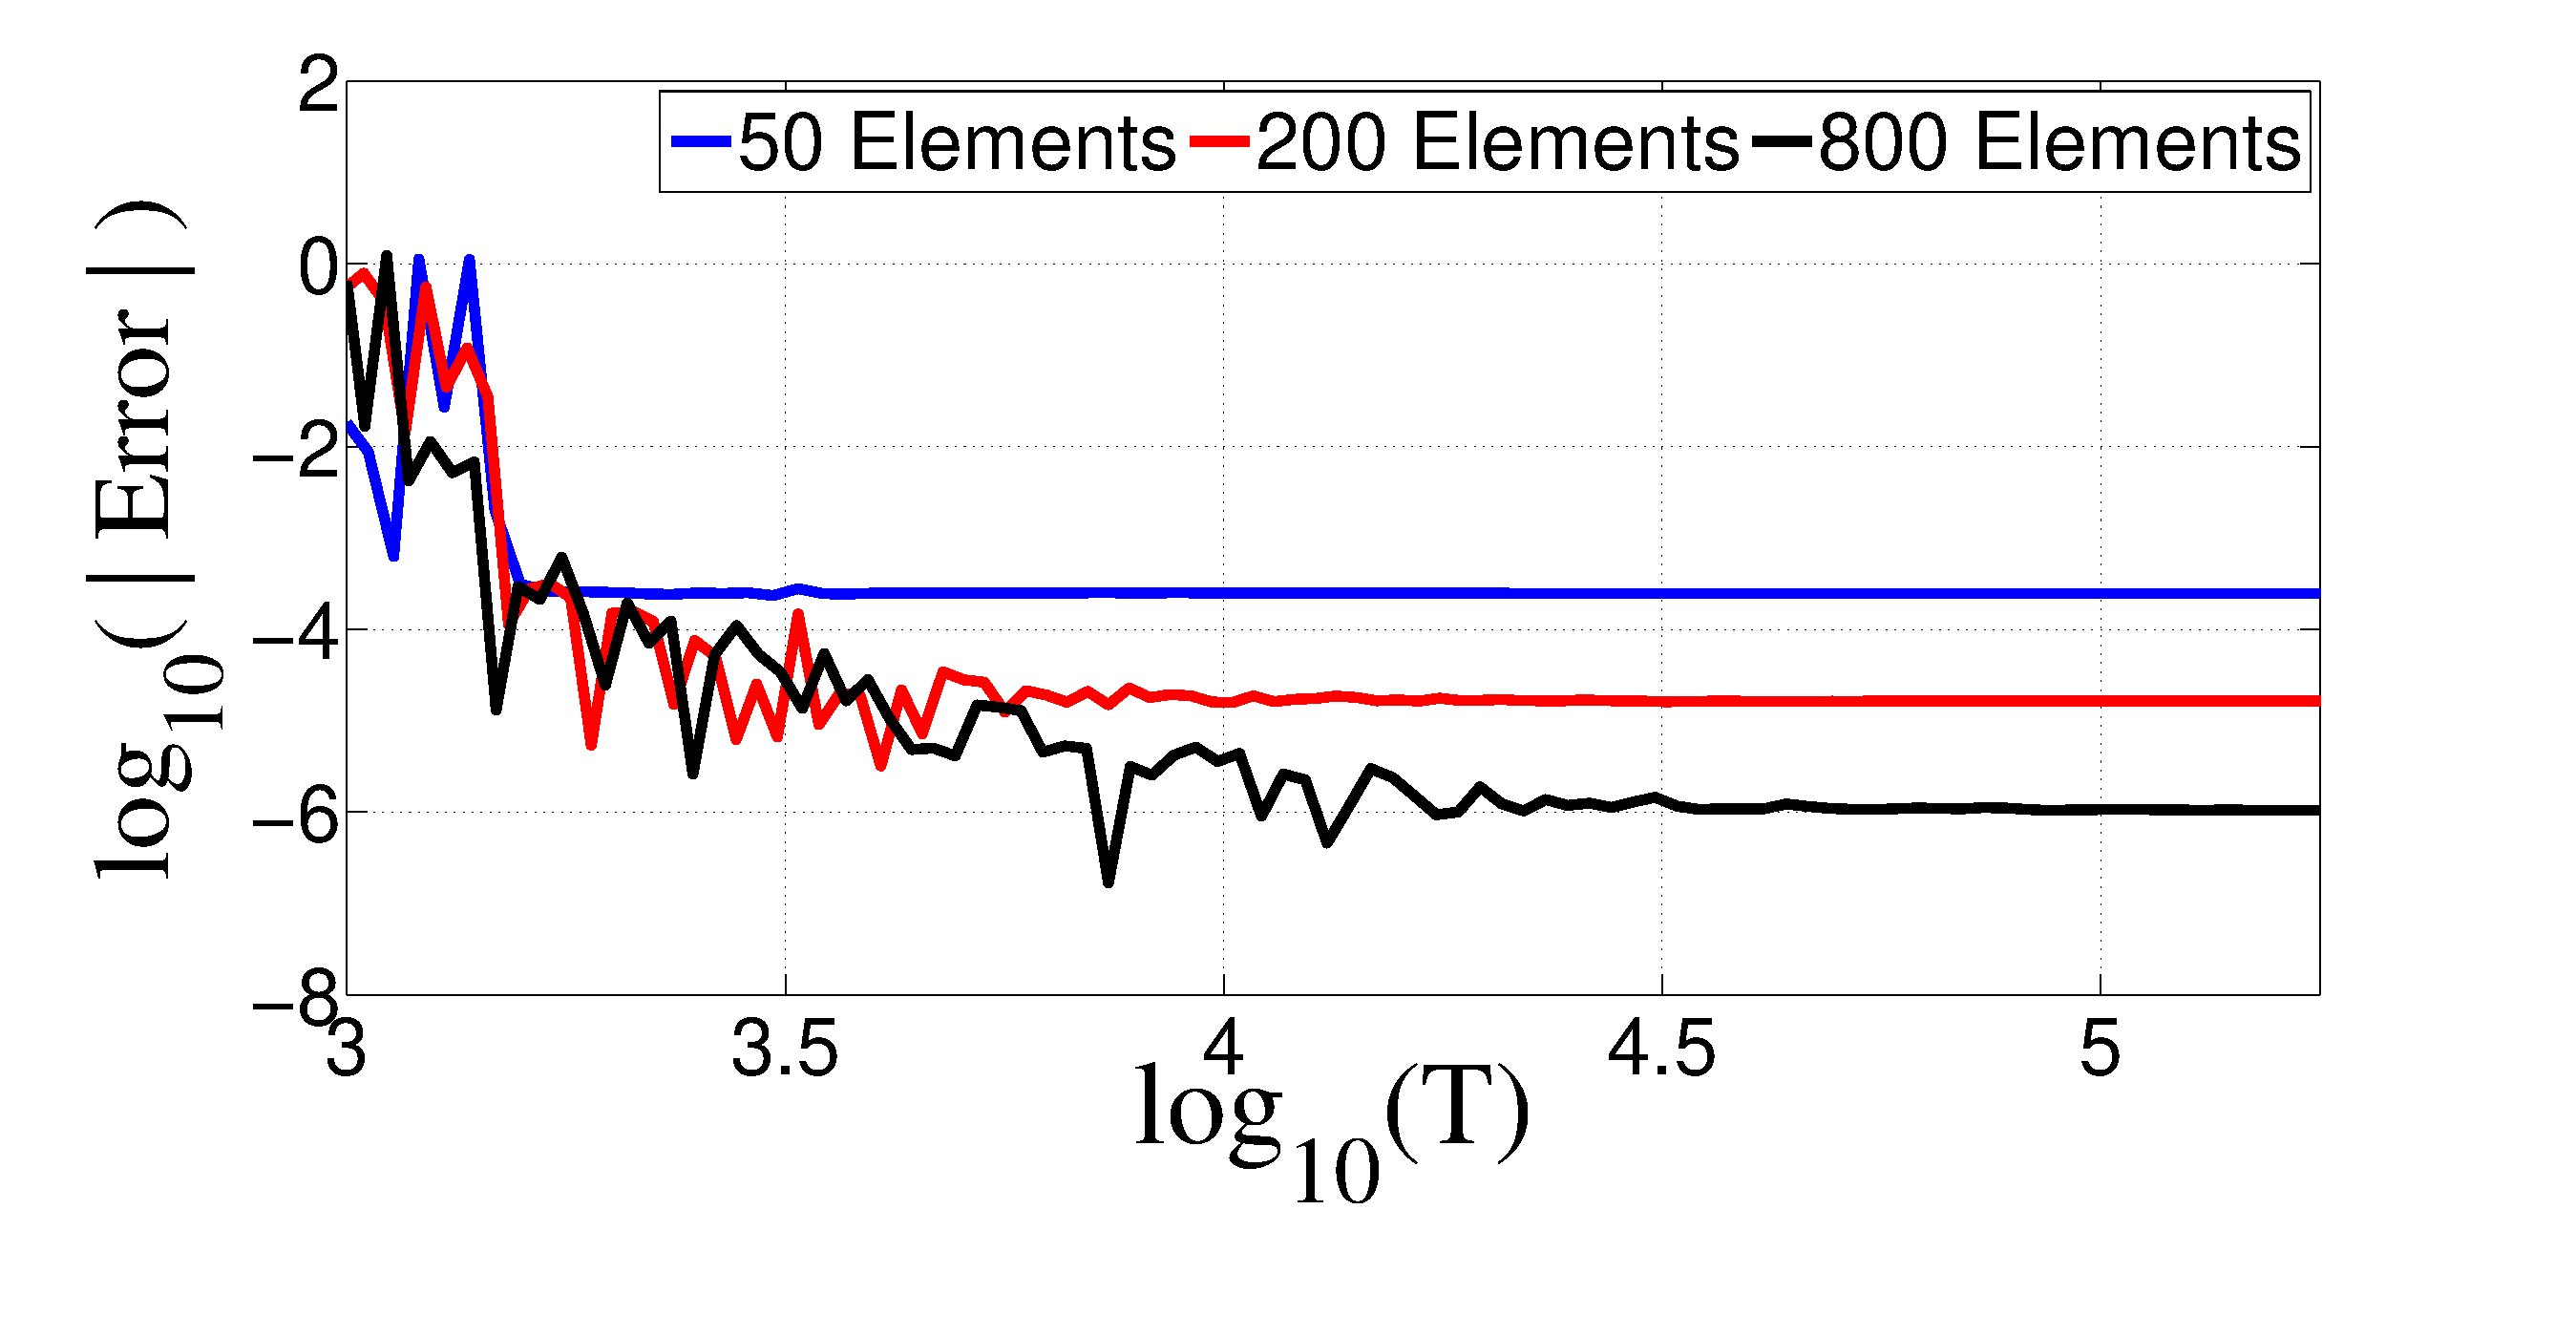
\includegraphics[width=0.75\textwidth]{Figures/FDMEvolutionWithPeriod/FDM_p1_U5_freq3_edited}
%     \label{freeSpaceConvergence}
%   }
% } \\
% \subfigure[]{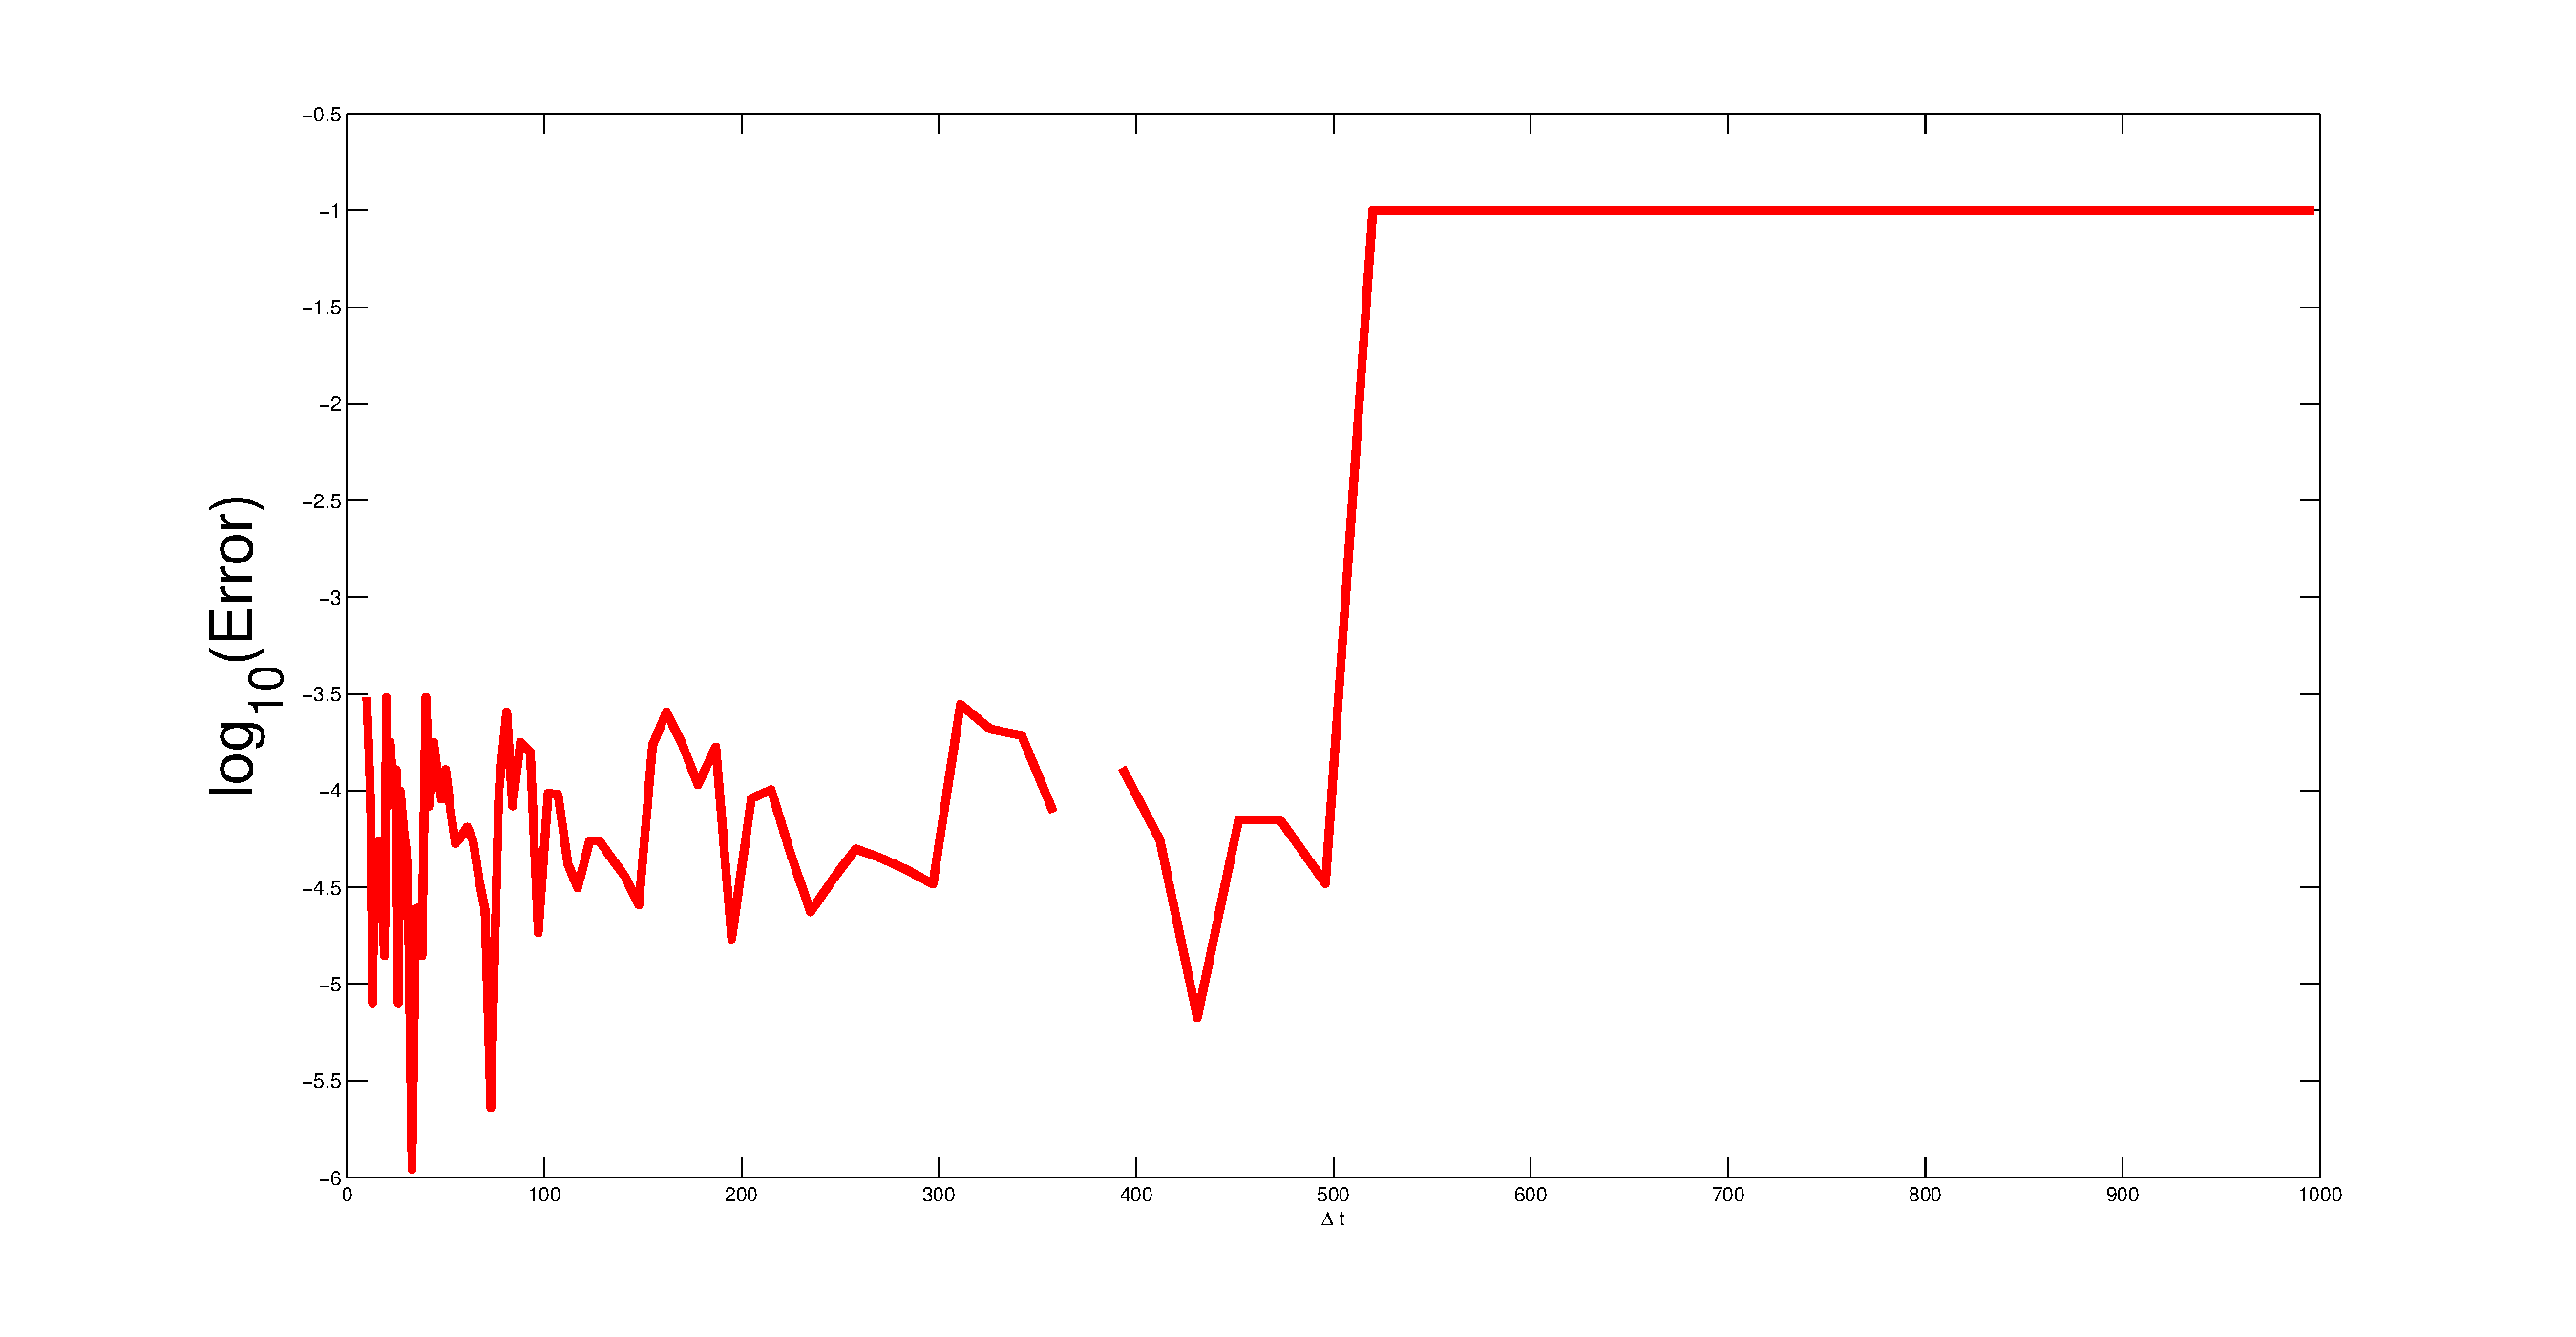
\includegraphics[width=0.3\textwidth]{Figures/dtRefinement/peakFreqError}} \\
% \end{tabular}

%\begin{tabular}{cc}
%\subfigure[A]{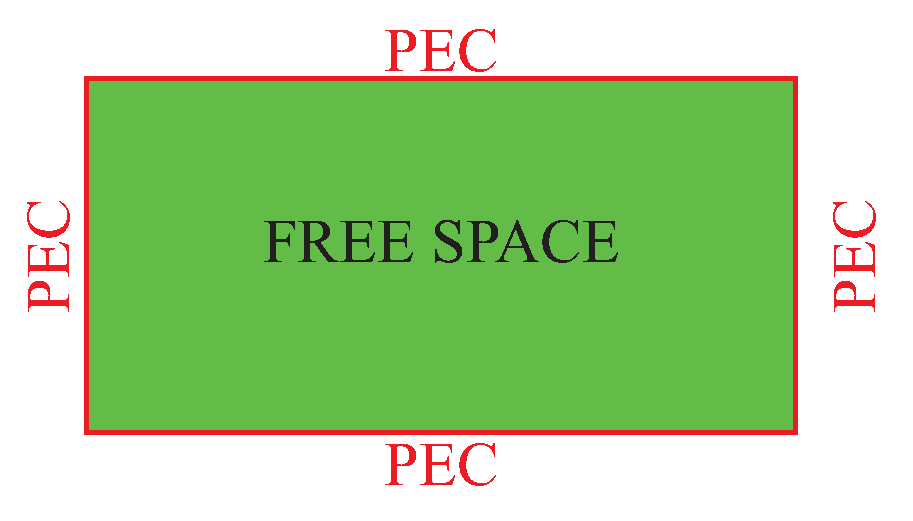
\includegraphics[width=0.3\textwidth]{Figures/Schematics/CavitySchematic}} & 
%\multirow{-2}[0]{*}{\subfigure[B]{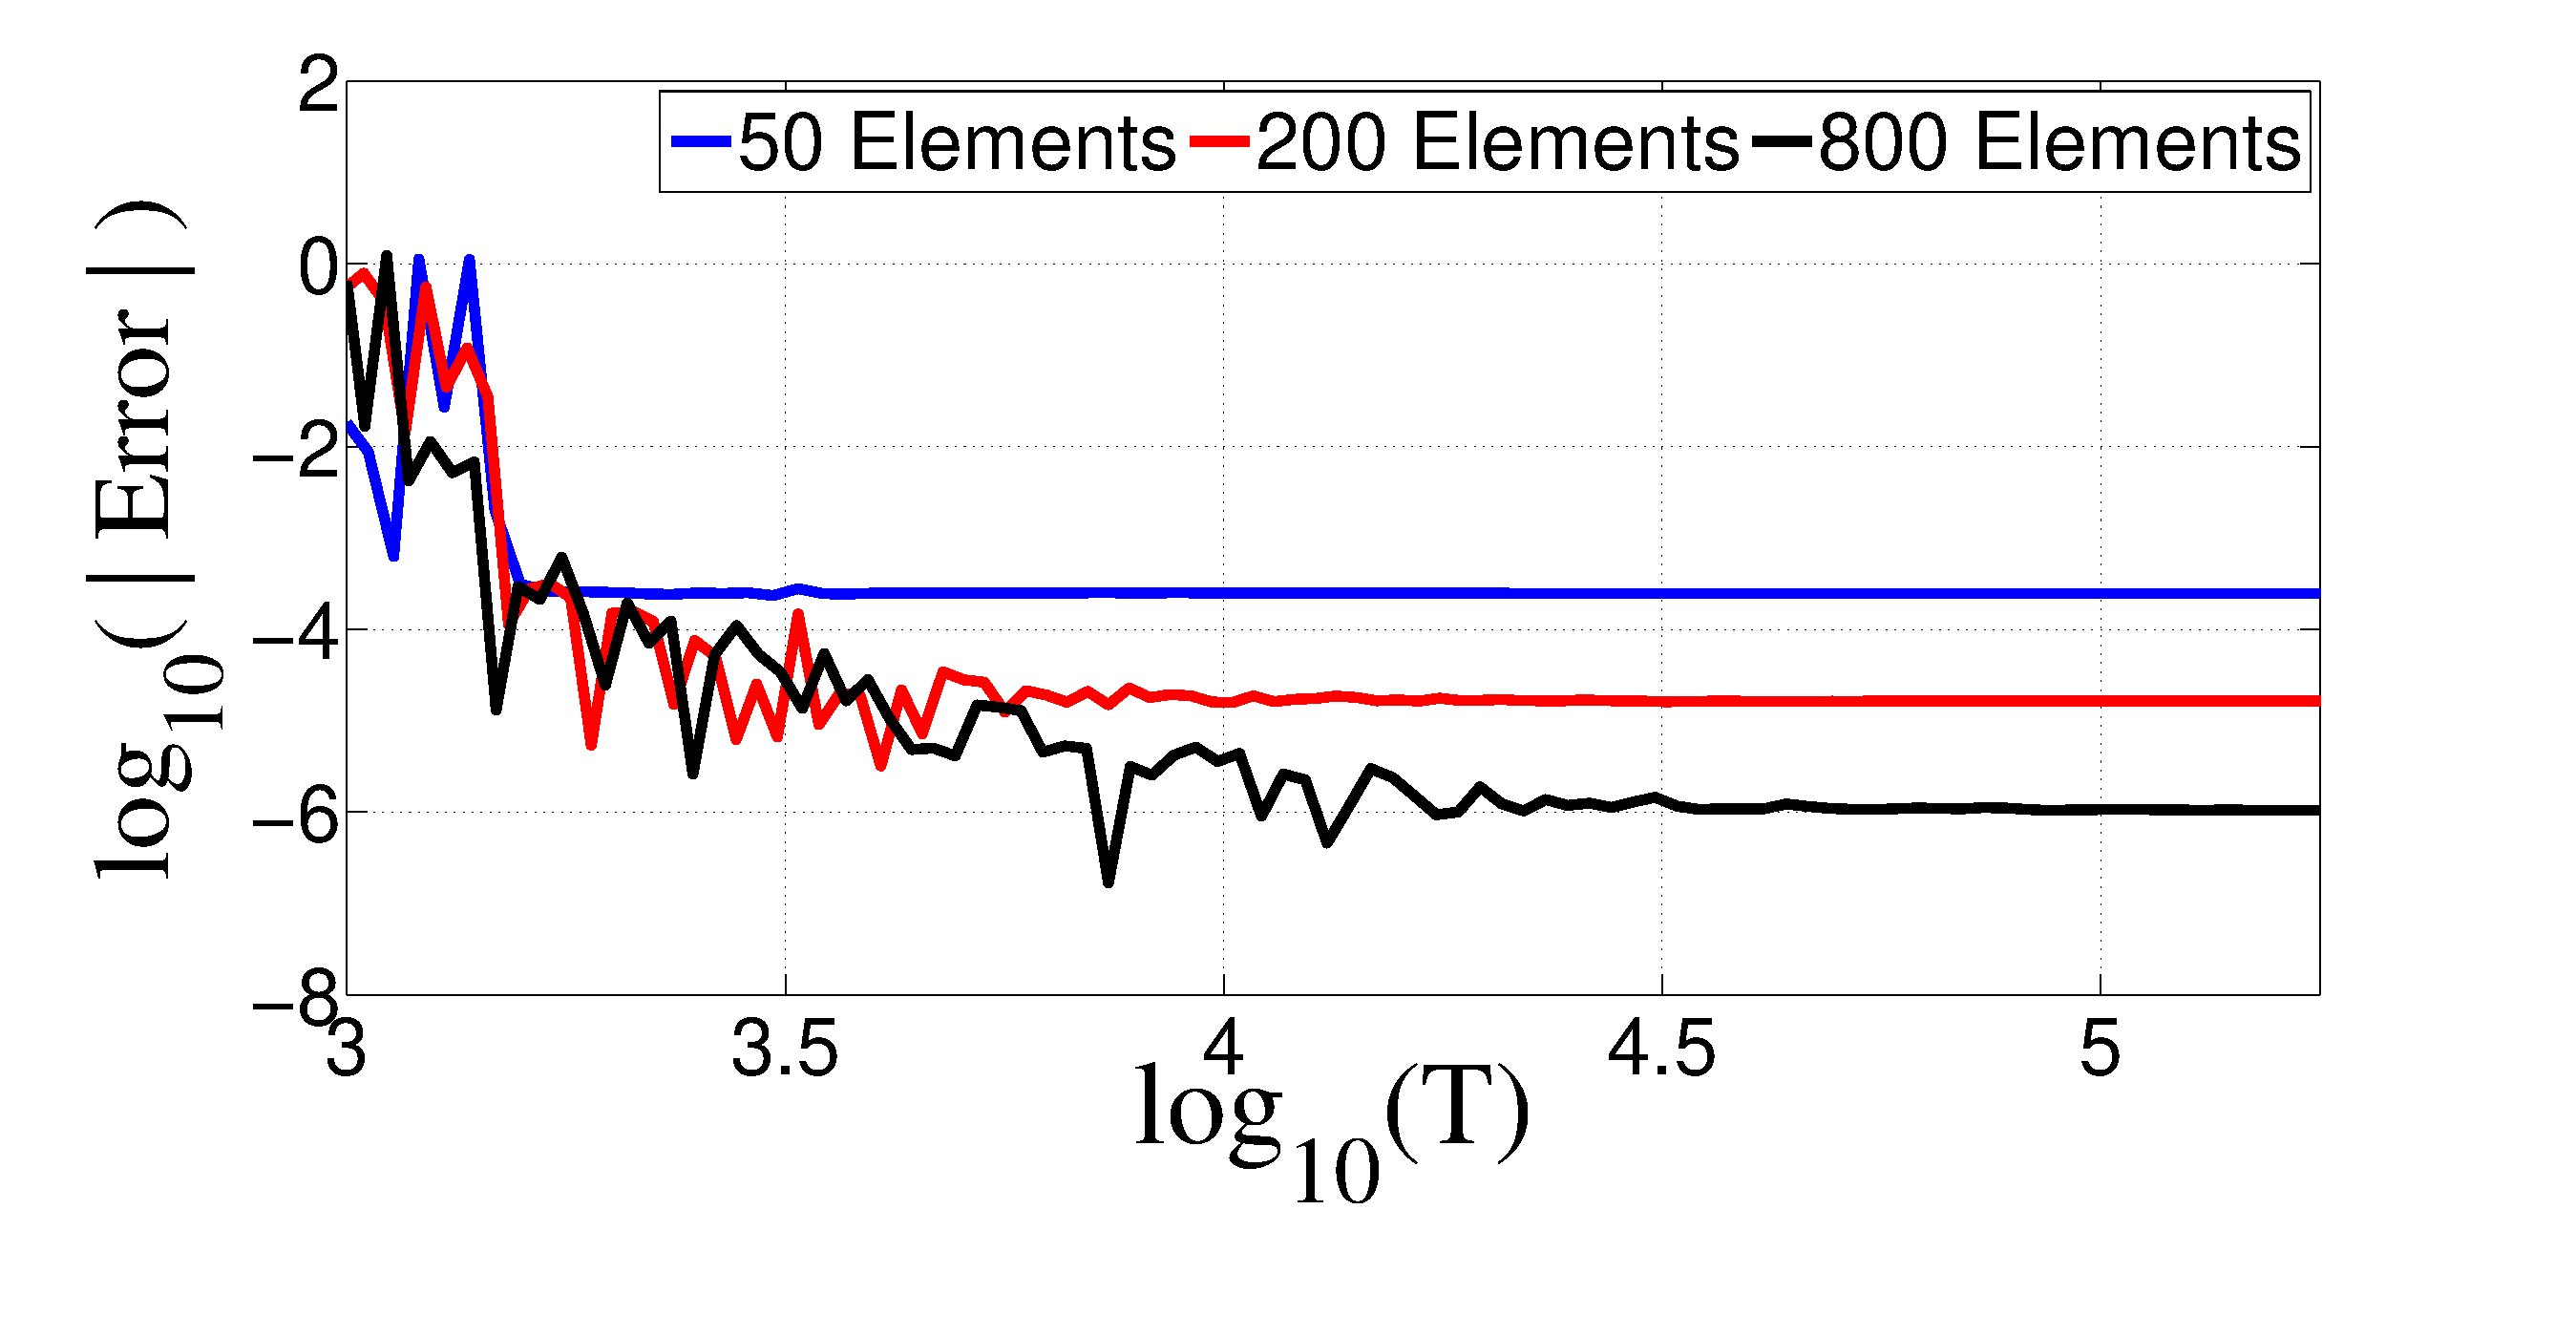
\includegraphics[width=0.7\textwidth]{Figures/FDMEvolutionWithPeriod/FDM_p1_U5_freq3_edited}} } \\
%\subfigure[C]{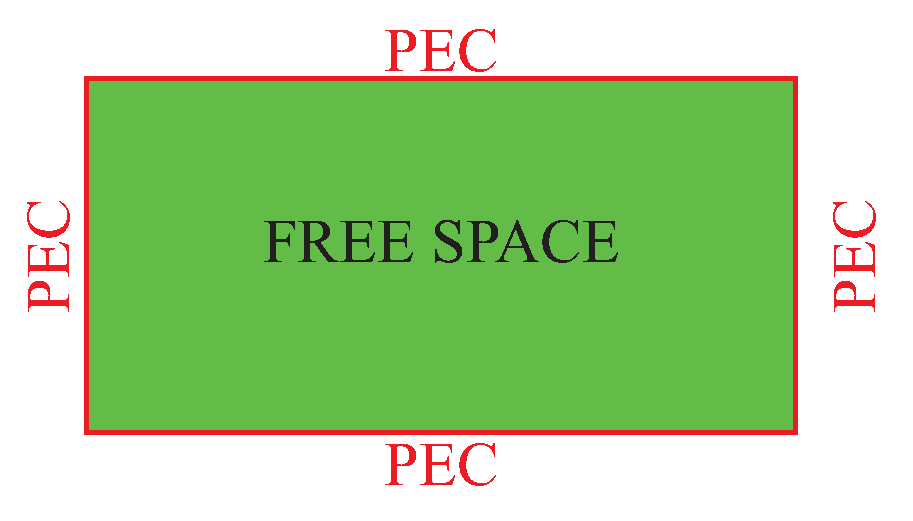
\includegraphics[width=0.3\textwidth]{Figures/Schematics/CavitySchematic}} \\
%\end{tabular}
%\caption{a) Schematic of free space cavity and PEC b) Convergence of relative error in resonant frequencies as the period T is increased for different mesh refinement in a free space cavity c) Relative error in resonant frequency with timestep $\Delta t$ }
%\end{figure}

%\begin{wrapfigure}{r}{0.4\textwidth}
% \centering
% 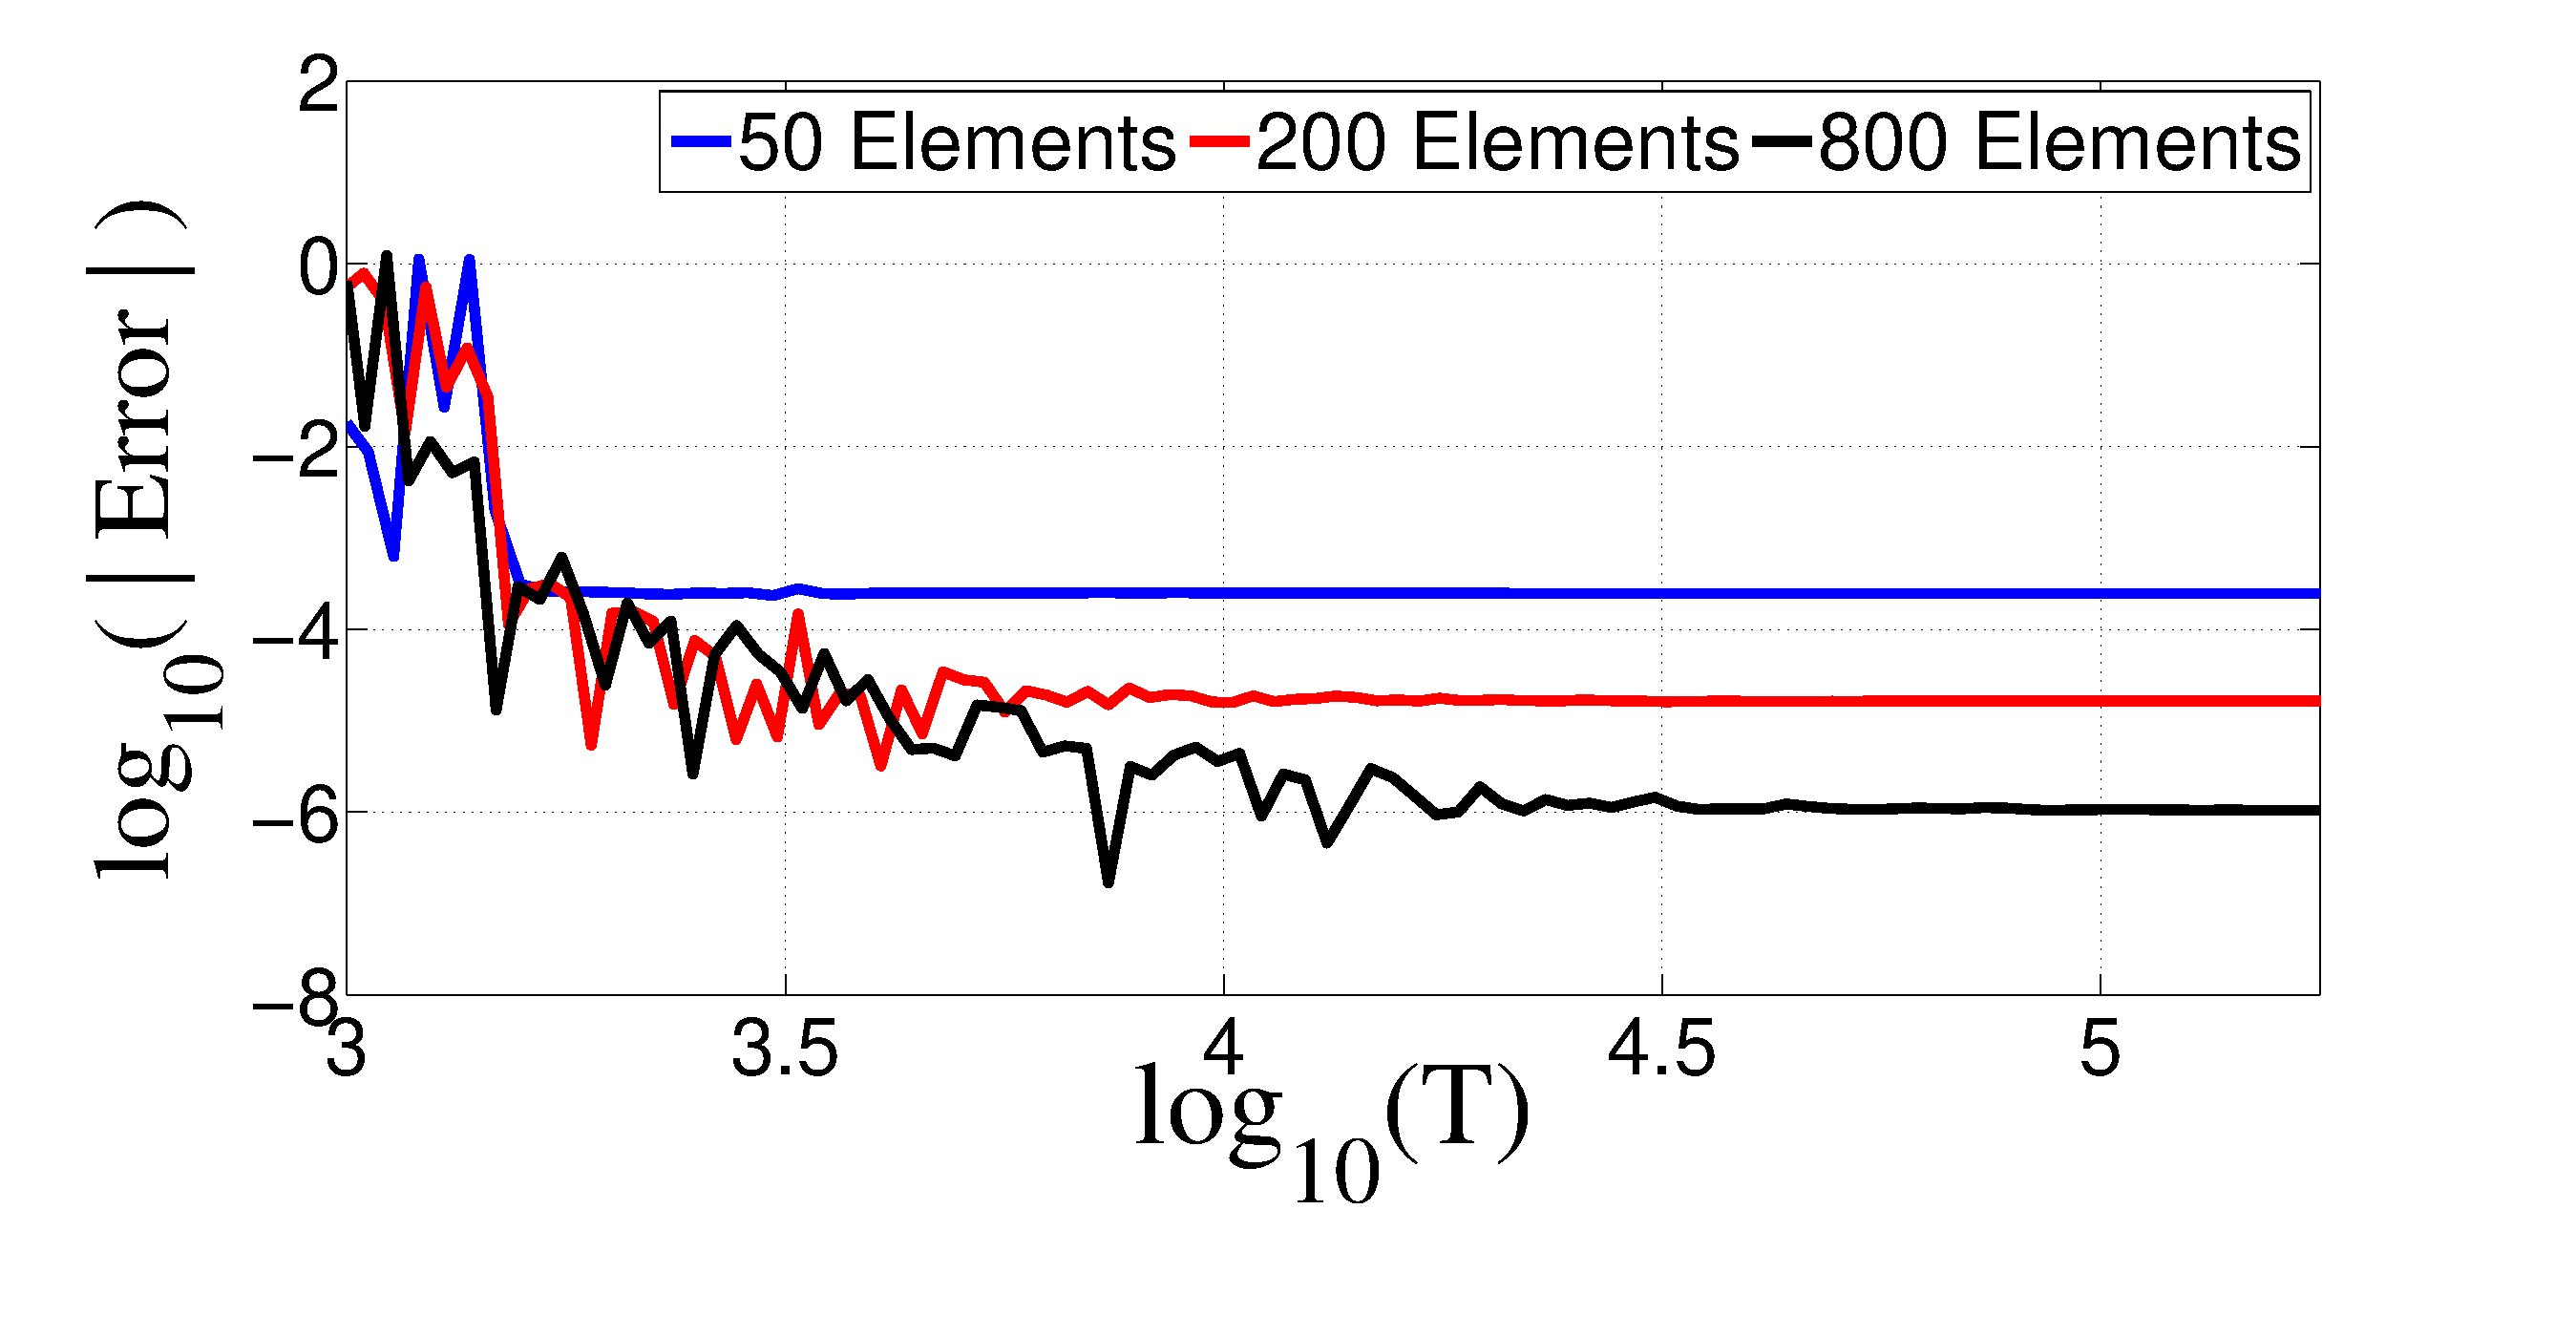
\includegraphics[width=0.35\textwidth]{Figures/FDMEvolutionWithPeriod/FDM_p1_U5_freq3_edited}
% \caption{Convergence of the calculated resonant frequencies to the known analytical solutions as the period T is increased for different mesh refinement in a free space cavity.}
% \label{freeSpaceConvergence}
%\end{wrapfigure}

%\subsection{Dispersive Cavity}

The second example presented is a dispersive cavity with an additional source term added to the right hand side of Maxwell's equations (\eqref{maxwell-eqtns}) to ensure that the problem has an exact known solution. The same 2D rectangular cavity as the previous example was considered filled with a gold medium ($\epsilon = 1, \sigma = 1, \omega = 6.7433, \gamma = 0.0799 $). Snapshots in time of the solutions obtained for the electric intensity vectors are shown in Figure \ref{dipersive-solution}.

\begin{figure}[htbp!]
 \centering
 \includegraphics[width=0.3\textwidth]{Figures/DispersiveCavityPlot/DispersiveCavityPlotE_1}
 \includegraphics[width=0.3\textwidth]{Figures/DispersiveCavityPlot/DispersiveCavityPlotE_2}
 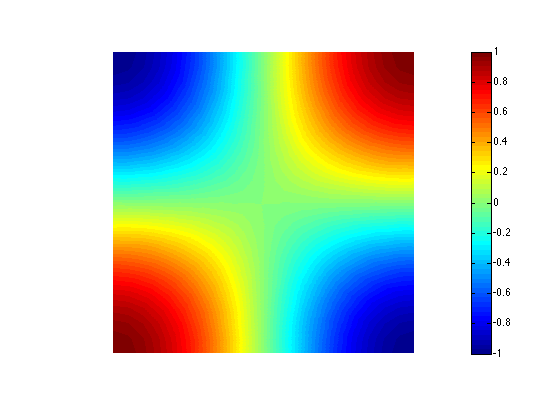
\includegraphics[width=0.3\textwidth]{Figures/DispersiveCavityPlot/DispersiveCavityPlotE_3}
 \caption{Left to right: Components $E_1$, $E_2$ and $E_3$ of the solution obtained for a rectangular cavity with a dispersive material and a volumetric source.}
 \label{dipersive-solution}
\end{figure}

Optimal convergence (i.e. a rate of $p + 1$ ) was achieved in the $\mathcal{L}^2(\Omega)$ norm of the relative error in the solution as shown in Figure \ref{dispersive-cavity-error} for component $E_1$.

\begin{figure}[htbp!]
 \centering
 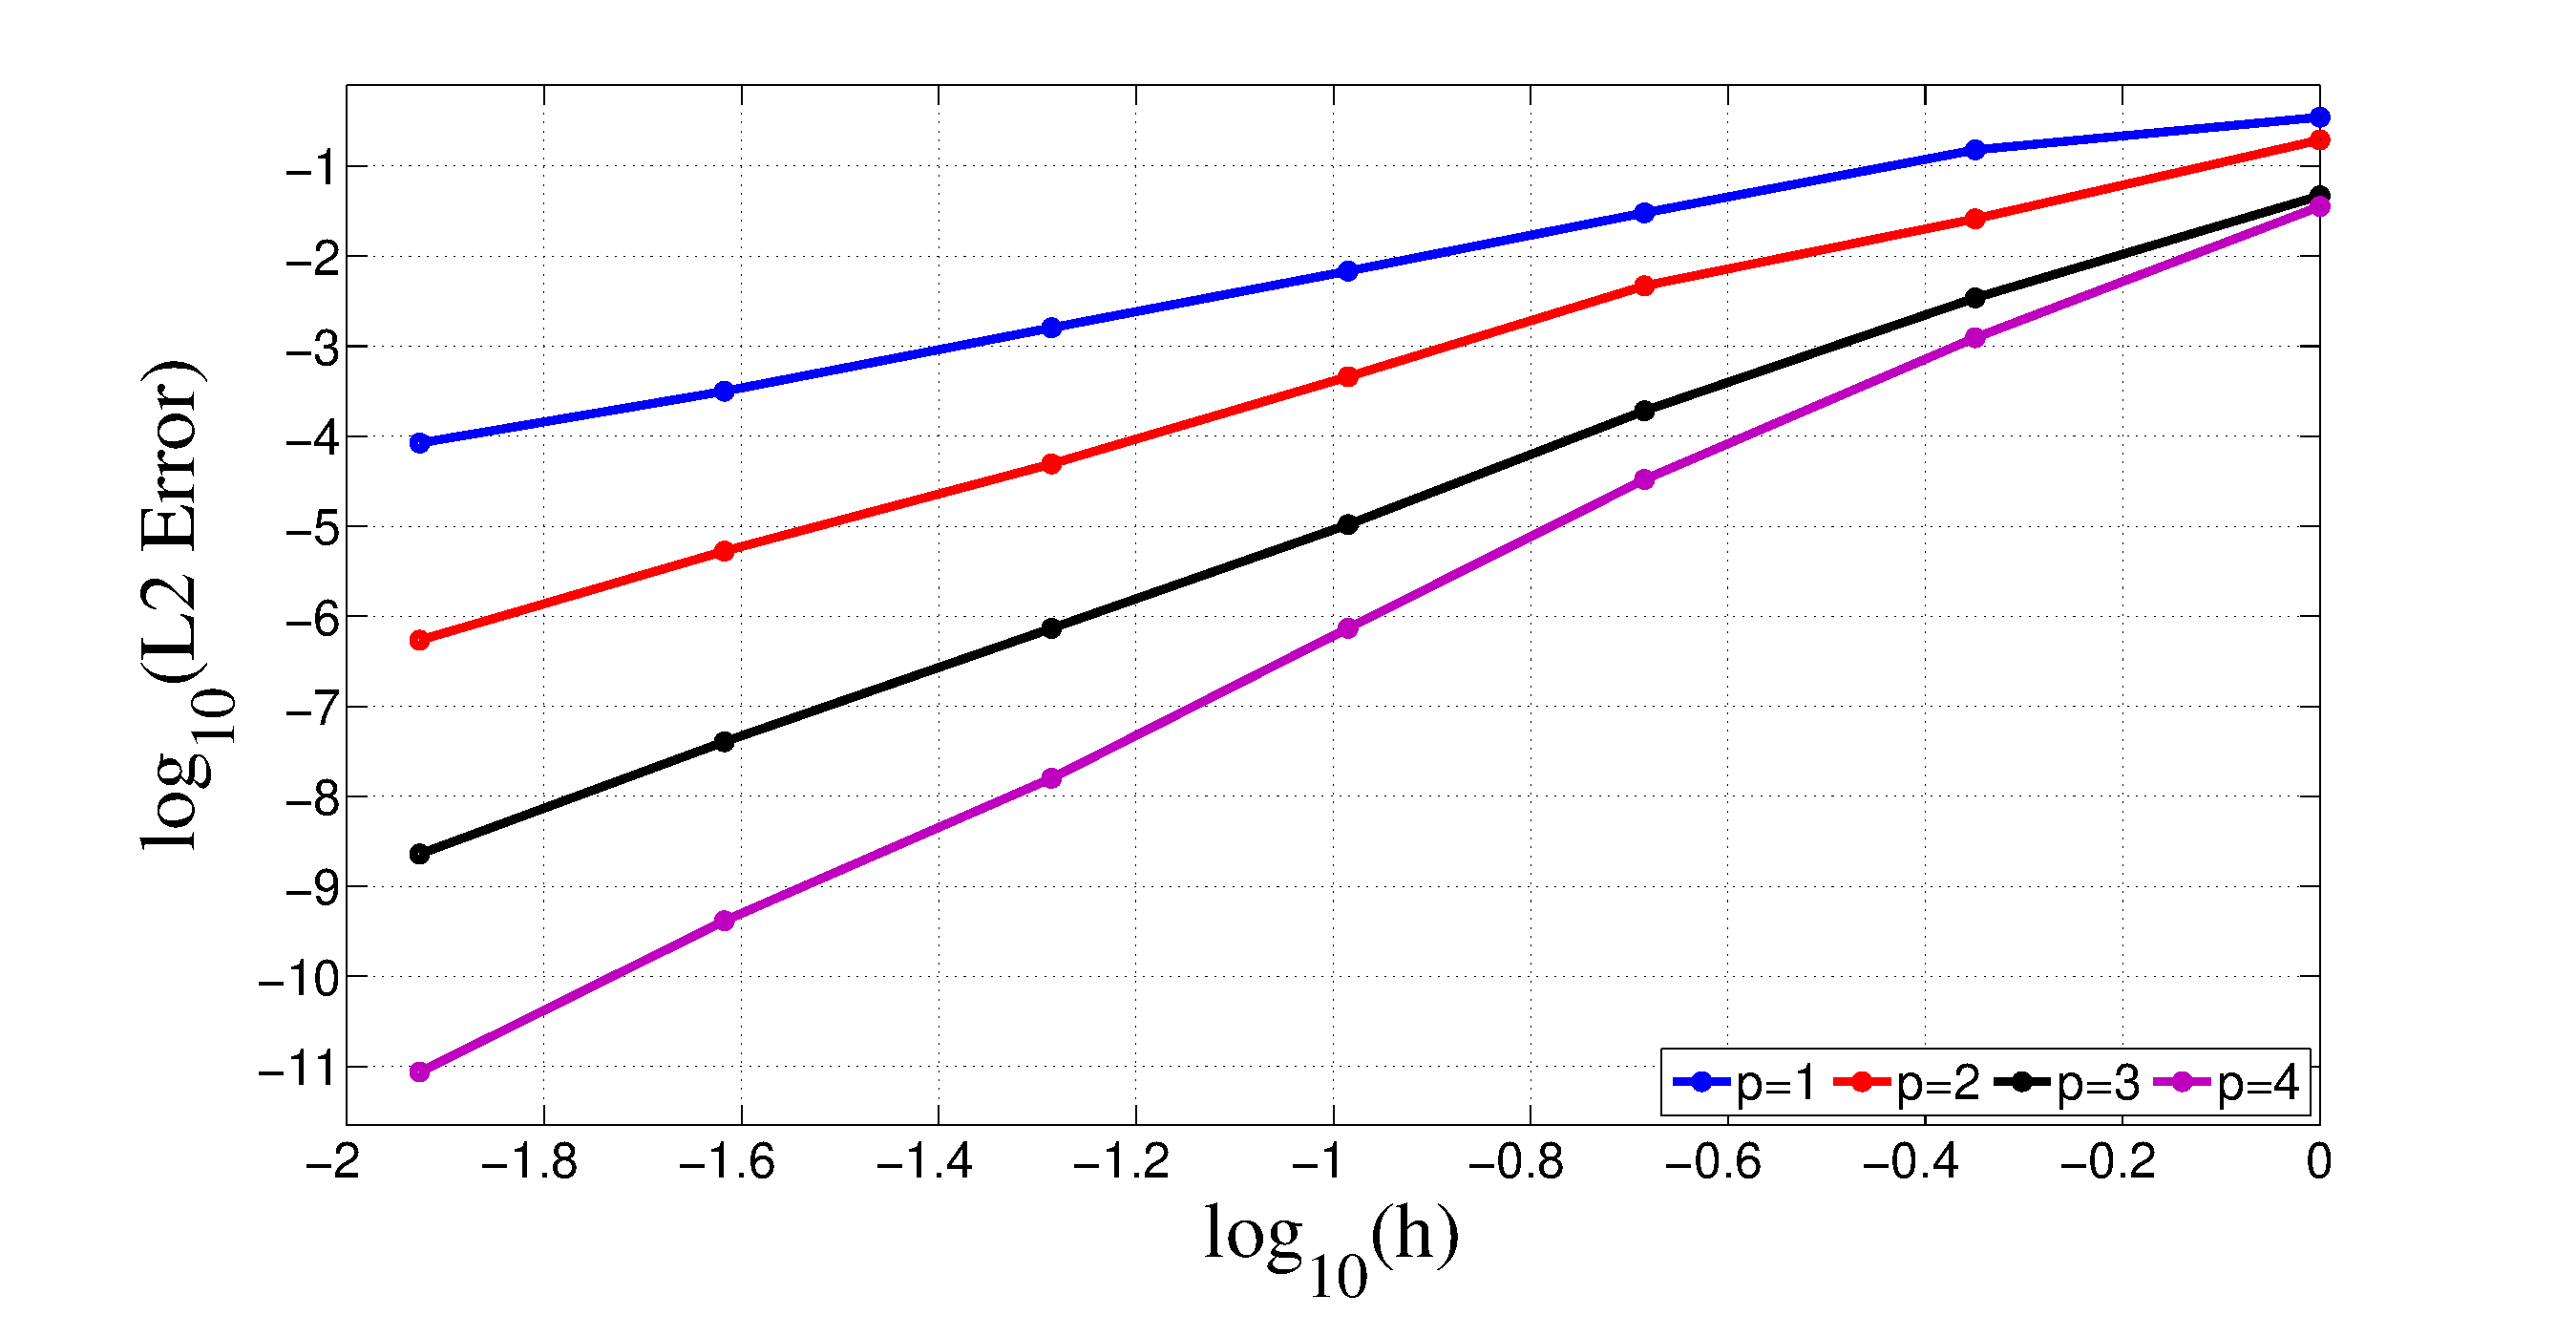
\includegraphics[height=6cm]{Figures/DispersiveValidationCase/convergenceAllComponents/L2vsH_TE_edited}
 \caption{$h$-convergence of the $\mathcal{L}^2(\Omega)$ norm of the relative error in $E_1$ for a cavity filled with dispersive material with an additional source term.}
 \label{dispersive-cavity-error}
\end{figure}

%\section{Achieving Frequency Resolution}

% Parallisation of the DG method can be attained with relative ease and allows the compution the evolution of the signal for an extended period of time.

%Parallisation of the DG code can be achieved by partitioning the physical domain into regions of adjacent elements with each processor performing computations on elements in a given region only. Since in the DG method calculations along faces involve values obtained from adjoining elements the values of the solution in neighbouring elements which are on other processors are communicated between each stage of the RK4 method.

% ** order of operations? - figure? ***

%The region calculated by each processor is selected to minimise the communication. Figure \ref{speed} shows the CPU time obtained as the number of nodes is increased.

% If communication was instantaneous we would expect doubling the number of processors to halve the computational time. In practice a limit is reached especially with smaller meshes where the communication dominates the behaviour and the additional speed up achieved by adding more processors is reduced. With smaller meshes this is especially true.

%\begin{figure}[htbp]
% \centering
% 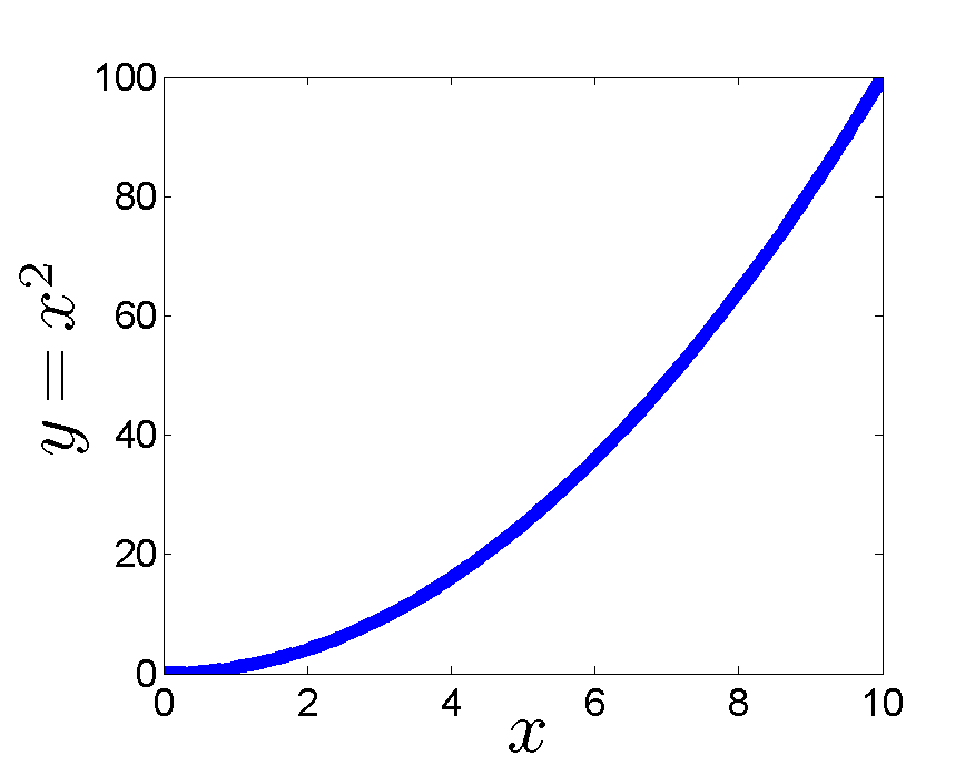
\includegraphics[height=7cm]{mypaper_example_graph}
% \caption{Cpu Times}
% \label{speed}
%\end{figure}
%
%Optimal convergence with mesh size was obtained for 3D parallelised code for high-order simulations with Pyramidal, Tetrahedral and *** elements and for 2D scattering from a circle with PML.

\section{Conclusions}

A method has been presented for obtaining frequency spectrum, resonant frequencies, mode shapes and quality factors for resonant cavities using a parallelised Discontinuous Galerkin time domain electromagnetic solver. Excellent agreement with analytical values has been observed for the resonant frequencies of a 2D free-space resonant cavity, and the convergence of the solution with the time period has been presented. The dispersive media implementation has been validated with the expected $h$-convergence of the $\mathcal{L}^2(\Omega)$ norm of the relative error.
%Finally, we present results for a realistic metal-coated semiconductor nanocylinder resonator.

\section*{Acknowledgements}\label{mypaper_sec:acknowledgements}

The authors gratefully acknowledge the financial support provided by the S\^{e}r Cymru National Research Network in Advanced Engineering and Materials

\nocite{*}
\bibliography{ACME2015-extendedAbstract}
\bibliographystyle{unsrt}

\end{document}